\chapter{Experimental Results and Analysis}
\label{chap:results}

This chapter presents the empirical evaluation of the contributions developed in Chapters~\ref{chap:evaluation-framework} to~\ref{chap:training-system}. It addresses a single question in stages: \emph{what is the strongest MicroRTS agent attainable under a realistic compute budget, and how does it perform against the established competition?}

The experiments build on one another. The network architecture is examined first (Section~\ref{sec:arch-sweep}), followed by an ablation of each training feature (Section~\ref{sec:feat-ablation}). The winning components of both studies feed into a full-scale single-map agent (Section~\ref{sec:single-map-agent}), which is then evaluated against the full competition pool (Section~\ref{sec:single-map-tournament}) and probed for robustness under distribution shift (Section~\ref{sec:gen-probes}). Two further experiments follow: Section~\ref{sec:bc-ppo} reports a standalone behavior-cloning warmstart study (BC-PPO), run separately from the main agent as a compute-efficiency comparison, and Section~\ref{sec:multi-map} builds a multi-map agent and contrasts it with the single-map specialist across the open layouts of size at most $16{\times}16$.
  
\vspace*{-0.1cm}

\section{Experimental Setup}
\label{sec:experimental-setup}

All experiments share the same PPO training stack, built on the MicroRTS environment described in Chapter~\ref{chap:python_bridge}. The baseline training configuration appears in Table~\ref{tab:baseline-setup}, and the corresponding hyperparameters in Table~\ref{tab:baseline-config}; together they serve as the reference for every subsequent experiment, and any deviation is stated explicitly. Evaluations use a fixed pool of scripted opponents with stochastic action sampling, under two protocols. Final checkpoint evaluations report win rates averaged over $1\,000$ games per opponent ($500$ as P0, $500$ as P1), giving balanced position coverage and statistically reliable estimates. In-training evaluations, run periodically during training to track learning dynamics, use a lighter protocol of $10$ games per opponent ($5$ as P0, $5$ as P1).

Several experiments ran concurrently on the high-performance computing (HPC) cluster. In particular, the feature ablation (Section~\ref{sec:feat-ablation}) overlapped with parts of the single-map training (Section~\ref{sec:single-map-agent}), so the latter could not retroactively incorporate every ablation finding. Sections are therefore ordered by logical dependency rather than chronological execution.

\vspace*{-0.1cm}

\begin{table}[H]
\centering
\caption[Baseline experiment setup]{Baseline experiment setup used throughout Chapter~\ref{chap:results} unless otherwise specified.\\PPO hyperparameters appear in Table~\ref{tab:baseline-config}.}
\label{tab:baseline-setup}
\small
\renewcommand{\arraystretch}{0.95}
\begin{tabularx}{\textwidth}{@{}l X@{}}
\toprule
\textbf{Parameter} & \textbf{Value} \\
\midrule
\multicolumn{2}{@{}l}{\textbf{\emph{Game environment}}}\\
Map                      & \textit{basesWorkers16x16A} ($16{\times}16$) \\
Max game length          & 4\,000 steps \\
\midrule
\multicolumn{2}{@{}l}{\textbf{\emph{Training opposition}}}\\
Environment setup        & 24 bot envs, diverse opponents, alternate players \\
Opponent distribution    & 9 CoacAI, 9 Mayari, 2 RandomBiasedAI, 2 WorkerRush, 2 LightRush \\
\midrule
\multicolumn{2}{@{}l}{\textbf{\emph{Reward signal}}}\\
Reward weights           & Default from Table~\ref{tab:reward-functions} \\
Value head               & shaped only \\
\midrule
\multicolumn{2}{@{}l}{\textbf{\emph{Hardware}}}\\
GPU                      & RTX 6000 Ada (48\,GB) \\
\bottomrule
\end{tabularx}
\end{table}

\paragraph*{Reproducibility and ethics.} All multi-seed experiments use the fixed seed set ${1, 2, 3}$ (the per-seed columns of the ablation tables correspond to these values); single-seed runs use seed~$1$. Every run executes on a single RTX~6000 Ada GPU ($48$ GB) and saves a self-contained \emph{config.json} for exact reconstruction, alongside the open-sourced codebase. The work involves no human subjects and no personal data; its only resource cost is compute, reported throughout in GPU-days.


\section{Architecture Ablation Analysis}
\label{sec:arch-sweep}

To isolate the effect of the network architecture, each candidate described in Table~\ref{tab:arch-summary} is trained under identical hyperparameters for $100$\,\text{M} environment steps on the same map. No advanced features are enabled, so any performance difference reflects architecture capacity alone. The full sweep ($7$ architectures $\times$ $3$ seeds at $100$\,\text{M} steps, $21$ runs) consumed $13.6$ GPU-days.

Table~\ref{tab:arch-ablation-summary} summarizes the mean win rate across three seeds for each architecture, with per-seed matchup breakdowns in Tables~\ref{tab:eval-1000games-s1}, \ref{tab:eval-1000games-s2}, and~\ref{tab:eval-1000games-s3}.

\begin{table}[!htp]
\centering
\caption[Architecture ablation: summary across seeds]{Architecture ablation summary across three seeds: mean overall win rate (\%) $\pm$ standard deviation, and mean improvement over baseline ($\bar{\Delta}$). Architectures sorted by mean overall win rate.}
\label{tab:arch-ablation-summary}
\small
\begin{tabular*}{\textwidth}{@{\extracolsep{\fill}}l | r r | c c c | c c@{}}
\toprule
\textbf{Architecture} & \textbf{Params} & \textbf{SPS} & \textbf{Seed 1} & \textbf{Seed 2} & \textbf{Seed 3} & \textbf{Mean $\pm$ Std} & \textbf{$\bar{\Delta}$ (pp)} \\
\midrule
GridNet                & 838\,\text{k}  & 2\,688 & 61.9 & 70.2 & 62.4 & 64.8 $\pm$ 3.8          & N/A \\
IMPALA-CNN             & 1.02\,\text{M} & 2\,416 & 73.4 & 60.5 & 72.1 & 68.7 $\pm$ 5.8          & \textcolor{teal}{+3.9} \\
IMPALA-CNN-Entity      & 1.37\,\text{M} & 1\,903 & 75.8 & 73.2 & 75.8 & 74.9 $\pm$ 1.2          & \textcolor{teal}{+10.1} \\
U-Net                  & 2.59\,\text{M} & 2\,121 & 77.9 & 78.4 & 74.8 & 77.0 $\pm$ 1.6          & \textcolor{teal}{+12.2} \\
U-Net-Entity-CBAM      & 2.90\,\text{M} & 1\,289 & 88.1 & 70.5 & 78.8 & 79.1 $\pm$ 7.2          & \textcolor{teal}{+14.3} \\
U-Net-Entity           & 2.90\,\text{M} & 1\,518 & 78.5 & 80.2 & 89.3 & 82.7 $\pm$ 4.7          & \textcolor{teal}{+17.9} \\
U-Net-Entity-CBAM-Deep & 4.72\,\text{M} & 1\,176 & 93.4 & 88.8 & 76.6 & \textbf{86.3 $\pm$ 7.1} & \textcolor{teal}{\textbf{+21.5}} \\
\bottomrule
\end{tabular*}
\end{table}

\begin{table}[!ht]
\centering
\footnotesize
\caption[Architecture ablation: per-seed win rates]{Architecture ablation per-seed: $1\,000$-game win rates. Each cell shows P0\,/\,P1 win rates~(\%). Overall = mean across opponents and positions. $\bar{\Delta}$ = improvement over \code{GridNet}.}
\label{tab:eval-1000games-perseed}

\begin{subtable}{\textwidth}
\subcaption{Seed 1}
\vspace{-0.15cm}
\label{tab:eval-1000games-s1}
\begin{tabularx}{\textwidth}{@{}l | *{5}{>{\centering\arraybackslash}X} | c c@{}}
\toprule
\textbf{Architecture} & \textbf{Random} & \textbf{WorkerRush} & \textbf{LightRush} & \textbf{CoacAI} & \textbf{Mayari} & \textbf{Overall} & \textbf{$\bar{\Delta}$ (pp)} \\
\midrule
GridNet                & 100.0\,/\,100.0 & 27.6\,/\,25.0 & 63.8\,/\,99.4 & 13.2\,/\,98.4 & 56.6\,/\,35.0 & 61.9\%          & N/A \\
IMPALA-CNN             & 100.0\,/\,100.0 & 99.2\,/\,79.8 & 98.6\,/\,67.6 & 18.8\,/\,30.6 & 74.6\,/\,64.4 & 73.4\%          & \textcolor{teal}{+11.5} \\
IMPALA-CNN-Entity      & 100.0\,/\,100.0 & 92.6\,/\,40.4 & 85.4\,/\,77.0 & 12.2\,/\,80.2 & 79.8\,/\,90.4 & 75.8\%          & \textcolor{teal}{+13.9} \\
U-Net                  & 100.0\,/\,100.0 & 81.0\,/\,80.2 & 82.0\,/\,99.4 & 18.0\,/\,96.4 & 79.6\,/\,42.6 & 77.9\%          & \textcolor{teal}{+16.0} \\
U-Net-Entity           & 100.0\,/\,100.0 & 35.2\,/\,99.6 & 63.0\,/\,49.8 & 72.4\,/\,73.4 & 98.0\,/\,94.0 & 78.5\%          & \textcolor{teal}{+16.6} \\
U-Net-Entity-CBAM      & 100.0\,/\,100.0 & 71.0\,/\,70.4 & 97.4\,/\,95.2 & 64.2\,/\,96.2 & 94.6\,/\,92.4 & 88.1\%          & \textcolor{teal}{+26.2} \\
U-Net-Entity-CBAM-Deep & 100.0\,/\,100.0 & 97.8\,/\,98.6 & 99.6\,/\,99.8 & 54.6\,/\,93.4 & 94.8\,/\,95.0 & \textbf{93.4\%} & \textcolor{teal}{\textbf{+31.5}} \\
\bottomrule
\end{tabularx}
\end{subtable}

\vspace{1em}

\begin{subtable}{\textwidth}
\subcaption{Seed 2}
\vspace{-0.15cm}
\label{tab:eval-1000games-s2}
\begin{tabularx}{\textwidth}{@{}l | *{5}{>{\centering\arraybackslash}X} | c c@{}}
\toprule
\textbf{Architecture} & \textbf{Random} & \textbf{WorkerRush} & \textbf{LightRush} & \textbf{CoacAI} & \textbf{Mayari} & \textbf{Overall} & \textbf{$\bar{\Delta}$ (pp)} \\
\midrule
IMPALA-CNN             & 100.0\,/\,100.0 & 56.6\,/\,10.4 & 86.8\,/\,75.4 & 20.8\,/\,38.6 & 70.0\,/\,46.2 & 60.5\%          & \textcolor{red}{$-$9.7} \\
GridNet                & 100.0\,/\,100.0 & 57.2\,/\,40.0 & 84.6\,/\,99.8 & 6.0\,/\,97.6  & 76.0\,/\,41.0 & 70.2\%          & N/A \\
U-Net-Entity-CBAM      & 100.0\,/\,100.0 & 97.8\,/\,74.4 & 74.2\,/\,96.8 & 0.6\,/\,27.6  & 55.2\,/\,78.4 & 70.5\%          & \textcolor{teal}{+0.3} \\
IMPALA-CNN-Entity      & 100.0\,/\,100.0 & 93.2\,/\,35.0 & 82.8\,/\,95.4 & 0.8\,/\,96.8  & 73.6\,/\,54.4 & 73.2\%          & \textcolor{teal}{+3.0} \\
U-Net                  & 100.0\,/\,100.0 & 85.4\,/\,97.0 & 91.6\,/\,96.4 & 15.4\,/\,65.4 & 76.0\,/\,56.8 & 78.4\%          & \textcolor{teal}{+8.2} \\
U-Net-Entity           & 100.0\,/\,100.0 & 97.4\,/\,99.8 & 96.8\,/\,100.0 & 0.4\,/\,98.0 & 90.4\,/\,19.4 & 80.2\%          & \textcolor{teal}{+10.0} \\
U-Net-Entity-CBAM-Deep & 100.0\,/\,100.0 & 95.0\,/\,99.4 & 97.4\,/\,100.0 & 23.4\,/\,93.4 & 86.8\,/\,92.6 & \textbf{88.8\%} & \textcolor{teal}{\textbf{+18.6}} \\
\bottomrule
\end{tabularx}
\end{subtable}

\vspace{1em}

\begin{subtable}{\textwidth}
\subcaption{Seed 3}
\vspace{-0.15cm}
\label{tab:eval-1000games-s3}
\begin{tabularx}{\textwidth}{@{}l | *{5}{>{\centering\arraybackslash}X} | c c@{}}
\toprule
\textbf{Architecture} & \textbf{Random} & \textbf{WorkerRush} & \textbf{LightRush} & \textbf{CoacAI} & \textbf{Mayari} & \textbf{Overall} & \textbf{$\bar{\Delta}$ (pp)} \\
\midrule
GridNet                & 100.0\,/\,100.0 & 43.2\,/\,31.8 & 68.8\,/\,96.4 & 2.2\,/\,83.8  & 71.8\,/\,26.2 & 62.4\%          & N/A \\
IMPALA-CNN             & 100.0\,/\,100.0 & 83.2\,/\,36.4 & 87.0\,/\,94.8 & 5.8\,/\,92.6  & 83.8\,/\,37.6 & 72.1\%          & \textcolor{teal}{+9.7} \\
U-Net                  & 100.0\,/\,100.0 & 92.8\,/\,71.4 & 89.0\,/\,99.8 & 0.8\,/\,98.4  & 70.4\,/\,25.6 & 74.8\%          & \textcolor{teal}{+12.4} \\
IMPALA-CNN-Entity      & 100.0\,/\,100.0 & 98.8\,/\,41.0 & 69.8\,/\,99.4 & 11.6\,/\,98.8 & 76.0\,/\,62.4 & 75.8\%          & \textcolor{teal}{+13.4} \\
U-Net-Entity-CBAM-Deep & 100.0\,/\,100.0 & 99.6\,/\,93.6 & 95.8\,/\,98.8 & 0.0\,/\,31.6  & 72.8\,/\,73.6 & 76.6\%          & \textcolor{teal}{+14.2} \\
U-Net-Entity-CBAM      & 100.0\,/\,100.0 & 93.6\,/\,48.0 & 96.2\,/\,99.8 & 0.2\,/\,98.0  & 85.6\,/\,66.8 & 78.8\%          & \textcolor{teal}{+16.4} \\
U-Net-Entity           & 100.0\,/\,100.0 & 99.8\,/\,97.4 & 92.4\,/\,87.0 & 42.2\,/\,85.2 & 98.6\,/\,90.8 & \textbf{89.3\%} & \textcolor{teal}{\textbf{+26.9}} \\
\bottomrule
\end{tabularx}
\end{subtable}

\end{table}

Cross-seed variance is substantial, up to $\pm7.2$ for the larger models. With only three seeds, several of the gaps below sit within the noise floor and cannot be resolved at this budget; the discussion therefore focuses on means and treats differences smaller than the seed-to-seed spread as \emph{inconclusive}. Rather than walking down the ranking row by row, the results are read through the three reasoning axes of Section~\ref{subsec:axes} (local spatial, long-range relational, and global spatial), asking for each how much it contributes and how reliably.

\subsection{Axis 1: Local Spatial Reasoning}

The three convolutional refinements of Section~\ref{sec:axis-local} target the local axis, the backbone onto which the relational and global modules are later added. Together they account for the largest share of the gain over \code{GridNet}, though their individual contributions vary in magnitude and reliability.

\paragraph*{Residual blocks (\code{IMPALA-CNN}, +3.9 pp).}

Replacing \code{GridNet}'s plain convolutions with \code{IMPALA-CNN} residual blocks shifts the mean from $64.8$ to $68.7$. The $+3.9$ pp gap overlaps with both seed-to-seed spreads ($\pm$3.8, $\pm5.8$), leaving the comparison inconclusive at this budget. Seed~1 hints that better gradient flow sharpens rush defense (WorkerRush $27.6\,/\,25.0$ $\to$ $99.2\,/\,79.8$) without affecting relational reasoning (CoacAI stays erratic). The value of residual blocks lies less in this modest gain than in enabling the deeper backbones below without unstable gradients.

\paragraph*{\code{U-Net} skips and SE attention (+12.2 pp over \code{GridNet}).}

Adding skip connections between encoder and decoder, plus SE channel attention, yields the largest local-axis jump ($64.8 \to 77.0$). The $+12.2$ pp gain is several times the seed-to-seed spread and one of the most consistent of the sweep ($\pm1.6$), so this contribution is robust. Preserving full-resolution detail through the bottleneck, rather than rebuilding it from a compressed code, repairs most of the P0/P1 asymmetry seen in skip-less architectures (seed~$1$: CoacAI P1 $30.6 \to 96.4$, LightRush P1 $67.6 \to 99.4$).

The residual asymmetry against CoacAI is non-architectural: replays show CoacAI placing its barracks at the bottom regardless of starting position, giving the agent a structural advantage as P1 (bottom spawn). The opponent's long-horizon economic strategies further demand counter-plans that no architecture reliably learns within the $100$\,\text{M}-step budget, even with CoacAI in the opponent pool: a budget or curriculum problem rather than an architectural one.

\paragraph*{CBAM spatial attention.}

CBAM adds a spatial gate on top of channel attention, selecting \emph{where} to attend, not just \emph{which} features matter. Its isolated effect is inconclusive at this scale: \code{U-Net-Entity} $\to$ \code{U-Net-Entity-CBAM} shifts the mean by $-3.6$ pp with the highest variance of the sweep ($\pm7.2$). Seed~$1$ is promising ($+9.6$ pp, removing the LightRush asymmetry $63.0\,/\,49.8$ $\to$ $97.4\,/\,95.2$), but seeds~$2$ and~$3$ fall back below \code{U-Net-Entity}. The gate seems constrained by limited capacity at this depth, with a clearer benefit emerging only once the network is deepened (Axis~$3$ below).

\subsection{Axis 2: Long-Range Relational Reasoning}

The Entity Transformer (Section~\ref{sec:axis-relational}) is the most reliable contribution in the sweep, adding value on top of \emph{either} backbone with consistent gains on the long-horizon, coordination-heavy opponents (CoacAI, Mayari) that the local axis alone does not solve. Relational reasoning therefore appears to complement rather than substitute for spatial capacity.

\paragraph*{On the \code{IMPALA-CNN} backbone (\code{IMPALA-CNN-Entity}, +6.2 pp).}
Adding the Transformer over extracted units to \code{IMPALA-CNN} lifts the mean from $68.7 \to 74.9$. The $+6.2$ pp gain exceeds both seed-to-seed spreads, and \code{IMPALA-CNN-Entity} is the most consistent architecture of the sweep ($\pm1.2$), making this contribution the most defensible of the study. All three seeds gain on the strategic bots (seed~1: CoacAI P1 $30.6 \to 80.2$, Mayari $74.6\,/\,64.4$ $\to$ $79.8\,/\,90.4$), at the cost of throughput ($2\,416 \to 1\,903$~SPS) and some rush defense (seed~$1$: WorkerRush P1 $79.8 \to 40.4$): the shared encoder reallocates capacity from spatial to relational features.

\paragraph*{On the \code{U-Net} backbone (\code{U-Net-Entity}, +5.7 pp).}
On \code{U-Net}, the same module yields a comparable $+5.7$ pp gain ($77.0 \to 82.7$), the second-best mean of the sweep, though higher variance ($\pm4.7$) brings the gap closer to the noise floor than on \code{IMPALA-CNN}. The spatial\,/\,relational tension persists: seed~1 gains Mayari $+18.4\,/\,+51.4$ but loses WorkerRush P0 ($81.0 \to 35.2$).

\vspace*{0.25cm}

This gain's reliability is structural, not a function of added capacity. Convolutions propagate interactions cell-by-cell through stacked receptive fields: two units far apart influence each other only after the signal traverses several layers of pooling and convolution. But in RTS, strategically meaningful interactions are entity-level: a worker and its base must coordinate as units, not spatial neighborhoods; a defender and the rusher it intercepts must reason about each other regardless of grid distance. Self-attention over entities bypasses spatial propagation: any two units are one attention hop apart. Hence a modest module (${\approx}\,$0.3\,\text{M} extra parameters) delivers a more reliable gain than far larger convolutional additions: the contribution is mechanistic, addressing reasoning convolutional capacity provides only at much higher parameter cost. More convolutional depth or width does not replace it, only approximates it inefficiently.

\subsection{Axis 3: Global Spatial Reasoning}

The final step adds the two global-axis mechanisms of Section~\ref{sec:axis-global}: bottleneck self-attention and a pyramidal depth profile $(2,3,4,3,2)$ that concentrates capacity where distant regions are summarized. Stacked onto \code{U-Net-Entity-CBAM}, they yield \code{U-Net-Entity-CBAM-Deep}, the top configuration by mean ($79.1 \to 86.3$, $+7.2$ pp, best seed $93.4$\%). The $+7.2$ pp gap, however, sits at roughly the $\pm7.1$ spread of the new architecture, so the improvement over \code{U-Net-Entity-CBAM} is suggestive rather than decisive. Two effects appear to combine. Depth supplies the capacity that the Axis~1 spatial gate lacked on its own, making CBAM effective in this deeper context. Global self-attention adds a complementary path, letting opposite ends of the map interact directly rather than through stacked receptive fields. Variance nonetheless stays high ($\pm7.1$; seed~$3$ CoacAI collapses to $0.0\,/\,31.6$): the added capacity sharpens the ceiling without removing the strategic blind spots.

\subsection{Final Architecture Choice}

Despite the high seed variance, \code{U-Net-Entity-CBAM-Deep} remains the most defensible choice for subsequent experiments. It covers all three reasoning axes, and the ablation attributes a non-negative contribution to each axis in the deep configuration, though CBAM's effect in isolation is inconclusive. It achieves the highest mean win rate ($86.3$\%) and the highest single-seed result ($93.4$\%). The variance ($\pm7.1$) likely reflects training stochasticity at 100\,\text{M} steps rather than an architectural limitation, though the 3-seed budget cannot rigorously establish this. The throughput cost ($1\,176$ vs $2\,688$~SPS for \code{GridNet}) is acceptable given the $+21.5$ pp improvement. The remainder of this chapter refers to this architecture as \code{UECD}.


\section{Feature Ablation Analysis}
\label{sec:feat-ablation}

Each feature is tested in isolation on top of the \code{UECD} baseline (Table~\ref{tab:baseline-setup}) for $50$\,\text{M} environment steps. This shorter budget keeps the total ablation compute within the available cluster allocation. Three independent seeds are run per configuration, providing a minimal estimate of run-to-run variance and a means of flagging features whose effect is dominated by noise. Each ablation row enables exactly one feature, or a tightly coupled pair that cannot be cleanly separated (e.g., \emph{filtered masks + reserved observations}). All other elements remain identical to the baseline: the network architecture, the optimization hyperparameters, the curriculum, and the evaluation protocol. The complete ablation consumed approximately $19.4$ GPU-days of training compute. 

\medskip

Table~\ref{tab:feat-ablation-summary} summarizes the mean win rate across the three seeds for each feature, with per-seed matchup breakdowns in Tables~\ref{tab:feat-ablation-s1}, \ref{tab:feat-ablation-s2}, and~\ref{tab:feat-ablation-s3}. Features are sorted by overall mean, and the baseline row separates features that help from those that hurt.

\medskip

Seed variance is wide enough that the table cannot be read as a clean ranking. The baseline alone carries a $\pm$7.5 standard deviation, and several features show $\pm$10 to $\pm$20 spreads, large enough that the gap between neighboring rows is usually smaller than the noise on each row.

\begin{table}[H]
\centering
\caption[Feature ablation: summary across seeds]{Feature ablation summary across three seeds: mean overall win rate (\%) $\pm$ standard deviation, mean pp improvement over baseline ($\bar{\Delta}$), and additional parameters relative to the baseline.}
\label{tab:feat-ablation-summary}
\small
\renewcommand{\arraystretch}{0.98}
\begin{tabularx}{\textwidth}{@{}l r | >{\centering\arraybackslash}X >{\centering\arraybackslash}X >{\centering\arraybackslash}X | c c@{}}
\toprule
\textbf{Feature} & \textbf{Add.\ Params} & \textbf{Seed 1} & \textbf{Seed 2} & \textbf{Seed 3} & \textbf{Mean $\pm$ Std} & \textbf{$\bar{\Delta}$ (pp)} \\
\midrule
  Extended Obs (73ch)            & $+$25.8\,\text{k}  & 83.6 & 86.7 & 82.7 & 84.3 $\pm$ 1.7 & \textcolor{teal}{+26.3} \\
  Filt.\ Masks + Res.\ Obs       & $+$560       & 85.9 & 83.1 & 72.8 & 80.6 $\pm$ 5.6 & \textcolor{teal}{+22.6} \\
  MCW                            & +0           & 77.8 & 78.7 & 78.6 & 78.4 $\pm$ 0.4 & \textcolor{teal}{+20.4} \\
  Opponent Modeling              & $+$10.5\,\text{k}  & 72.4 & 78.9 & 82.1 & 77.8 $\pm$ 4.0 & \textcolor{teal}{+19.8} \\
  Triple Value Heads             & $+$137.7\,\text{k} & 77.6 & 72.6 & 67.9 & 72.7 $\pm$ 4.0 & \textcolor{teal}{+14.7} \\
  PAE (keep=95\%)                & +0           & 67.6 & 63.8 & 82.4 & 71.3 $\pm$ 8.0 & \textcolor{teal}{+13.3} \\
  Hierarchical Mask              & +0           & 59.9 & 66.4 & 86.8 & 71.1 $\pm$ 11.5 & \textcolor{teal}{+13.1} \\
  Adaptive Opponents             & +0           & 67.9 & 69.6 & 71.4 & 69.6 $\pm$ 1.4 & \textcolor{teal}{+11.7} \\
  PopArt                         & +0           & 65.5 & 59.7 & 80.4 & 68.5 $\pm$ 8.7 & \textcolor{teal}{+10.6} \\
  Aux Unit Count                 & $+$3.9\,\text{k}   & 83.6 & 66.2 & 52.9 & 67.6 $\pm$ 12.6 & \textcolor{teal}{+9.6} \\
  Bots + Self-Play + PFSP        & +0           & 58.9 & 79.6 & 62.2 & 66.9 $\pm$ 9.1 & \textcolor{teal}{+8.9} \\
  GELU                           & +0           & 69.6 & 74.3 & 55.0 & 66.3 $\pm$ 8.2 & \textcolor{teal}{+8.3} \\
  Frame Stack (4)                & $+$45.4\,\text{k}  & 71.4 & 64.3 & 60.4 & 65.3 $\pm$ 4.5 & \textcolor{teal}{+7.3} \\
  Autoregressive + Hier.\ Mask   & $+$28.2\,\text{k}  & 59.1 & 60.4 & 75.9 & 65.1 $\pm$ 7.6 & \textcolor{teal}{+7.2} \\
  Autoregressive                 & $+$28.2\,\text{k}  & 70.7 & 53.2 & 67.3 & 63.7 $\pm$ 7.6 & \textcolor{teal}{+5.8} \\
  Aux Spatial                    & $+$1.2\,\text{k}   & 56.1 & 68.3 & 65.4 & 63.3 $\pm$ 5.2 & \textcolor{teal}{+5.3} \\
  SPP Critic                     & $+$81.9\,\text{k}  & 74.8 & 58.6 & 56.2 & 63.2 $\pm$ 8.3 & \textcolor{teal}{+5.2} \\
  Aux Contrastive                & $+$22.8\,\text{k}  & 70.6 & 54.8 & 59.5 & 61.6 $\pm$ 6.6 & \textcolor{teal}{+3.7} \\
  Build-Time Rewards             & +0           & 46.9 & 62.3 & 74.3 & 61.2 $\pm$ 11.2 & \textcolor{teal}{+3.2} \\
\midrule
  \textbf{Baseline}              & N/A         & 50.4 & 55.3 & 68.2 & 58.0 $\pm$ 7.5 & N/A \\
\midrule
  Augment Symmetry               & +0           & 62.6 & 56.9 & 52.9 & 57.5 $\pm$ 4.0 & \textcolor{red}{$-$0.5} \\
  HL-Gauss                       & $+$16.5\,\text{k}  & 62.2 & 21.2 & 35.0 & 39.5 $\pm$ 17.0 & \textcolor{red}{$-$18.5} \\
\bottomrule
\end{tabularx}
\end{table}

\begin{table}[H]
\centering
\footnotesize
\caption[Feature ablation: per-seed win rates]{Feature ablation per-seed: $1\,000$-game win rates. Each cell shows P0\,/\,P1 win rates~(\%). Overall = mean across opponents and positions. $\Delta$ = pp improvement over baseline.}
\label{tab:feat-ablation-perseed}

\begin{subtable}{\textwidth}
\subcaption{Seed 1}
\label{tab:feat-ablation-s1}
\vspace{-0.15cm}
\begin{tabularx}{\textwidth}{@{}l | *{5}{>{\centering\arraybackslash}X} | c c@{}}
\toprule
\textbf{Feature} & \textbf{Random} & \textbf{WorkerRush} & \textbf{LightRush} & \textbf{CoacAI} & \textbf{Mayari} & \textbf{Overall} & \textbf{$\Delta$ (pp)} \\
\midrule
Filt.\ Masks + Res.\ Obs       & 100.0\,/\,100.0 & 67.2\,/\,88.8 & 99.4\,/\,66.0 & 59.4\,/\,89.0 & 89.4\,/\,99.6 & 85.9\% & \textcolor{teal}{+35.5} \\
Extended Obs (73ch)            & 100.0\,/\,100.0 & 67.6\,/\,75.2 & 99.2\,/\,100.0  & 22.8\,/\,81.2 & 95.6\,/\,94.6 & 83.6\% & \textcolor{teal}{+33.2} \\
Aux Unit Count                 & 100.0\,/\,100.0 & 82.4\,/\,96.2 & 92.8\,/\,99.0 & 30.6\,/\,76.6 & 78.6\,/\,80.2 & 83.6\% & \textcolor{teal}{+33.2} \\
MCW                            & 100.0\,/\,100.0 & 71.2\,/\,92.2 & 84.0\,/\,99.0 & 21.2\,/\,84.8 & 67.8\,/\,57.6 & 77.8\% & \textcolor{teal}{+27.4} \\
Triple Value Heads             & 100.0\,/\,100.0 & 41.8\,/\,76.2 & 98.4\,/\,98.4 & 28.4\,/\,80.6 & 94.0\,/\,58.0 & 77.6\% & \textcolor{teal}{+27.2} \\
SPP Critic                     & 100.0\,/\,100.0 & 43.8\,/\,46.4 & 99.4\,/\,97.2 & 24.0\,/\,85.6 & 80.2\,/\,71.8 & 74.8\% & \textcolor{teal}{+24.4} \\
Opponent Modeling              & 100.0\,/\,100.0 & 98.2\,/\,37.4 & 96.2\,/\,88.0 & 13.2\,/\,60.6 & 79.6\,/\,50.4 & 72.4\% & \textcolor{teal}{+22.0} \\
Frame Stack (4)                & 100.0\,/\,100.0 & 97.8\,/\,55.6 & 90.6\,/\,93.8 & 0.0\,/\,53.8  & 70.8\,/\,51.2 & 71.4\% & \textcolor{teal}{+21.0} \\
Autoregressive                 & 100.0\,/\,100.0 & 62.6\,/\,59.0 & 81.2\,/\,82.0 & 17.0\,/\,67.8 & 82.0\,/\,55.6 & 70.7\% & \textcolor{teal}{+20.3} \\
Aux Contrastive                & 100.0\,/\,100.0 & 81.8\,/\,39.0 & 59.8\,/\,45.6 & 49.8\,/\,64.0 & 88.4\,/\,77.4 & 70.6\% & \textcolor{teal}{+20.2} \\
GELU                           & 100.0\,/\,100.0 & 46.4\,/\,31.8 & 93.4\,/\,97.6 & 40.4\,/\,85.2 & 73.6\,/\,28.0 & 69.6\% & \textcolor{teal}{+19.2} \\
Adaptive Opponents             & 100.0\,/\,100.0 & 63.4\,/\,55.8 & 85.8\,/\,90.8 & 10.8\,/\,70.6 & 59.8\,/\,41.8 & 67.9\% & \textcolor{teal}{+17.5} \\
PAE (keep=95\%)                & 100.0\,/\,100.0 & 26.8\,/\,92.2 & 10.4\,/\,97.4 & 4.0\,/\,91.0  & 69.2\,/\,84.6 & 67.6\% & \textcolor{teal}{+17.2} \\
PopArt                         & 100.0\,/\,100.0 & 70.8\,/\,62.0 & 53.0\,/\,99.4 & 0.0\,/\,77.0  & 33.4\,/\,59.2 & 65.5\% & \textcolor{teal}{+15.1} \\
Augment Symmetry               & 100.0\,/\,100.0 & 31.2\,/\,22.2 & 46.0\,/\,84.8 & 23.4\,/\,79.6 & 79.2\,/\,59.2 & 62.6\% & \textcolor{teal}{+12.2} \\
HL-Gauss                       & 100.0\,/\,100.0 & 44.6\,/\,48.8 & 49.4\,/\,27.8 & 35.0\,/\,44.6 & 90.2\,/\,81.4 & 62.2\% & \textcolor{teal}{+11.8} \\
Hierarchical Mask              & 100.0\,/\,100.0 & 69.2\,/\,14.8 & 90.4\,/\,96.4 & 0.2\,/\,4.6   & 64.4\,/\,59.2 & 59.9\% & \textcolor{teal}{+9.5} \\
Autoregressive + Hier.\ Mask   & 100.0\,/\,100.0 & 83.8\,/\,24.0 & 78.2\,/\,55.4 & 8.0\,/\,27.4  & 66.0\,/\,48.2 & 59.1\% & \textcolor{teal}{+8.7} \\
Bots + Self-Play + PFSP        & 100.0\,/\,100.0 & 43.8\,/\,36.2 & 84.0\,/\,80.6 & 6.6\,/\,28.0  & 64.6\,/\,44.8 & 58.9\% & \textcolor{teal}{+8.5} \\
Aux Spatial                    & 100.0\,/\,100.0 & 66.2\,/\,15.4 & 70.0\,/\,76.4 & 13.2\,/\,21.6 & 56.2\,/\,42.0 & 56.1\% & \textcolor{teal}{+5.7} \\
\midrule
\textbf{Baseline}              & 100.0\,/\,100.0 & 42.4\,/\,23.4 & 96.8\,/\,51.2 & 0.0\,/\,0.0       & 75.4\,/\,14.6 & 50.4\% & N/A \\
\midrule
Build-Time Rewards             & 100.0\,/\,100.0 & 24.0\,/\,9.0  & 41.2\,/\,19.0 & 27.6\,/\,29.2 & 68.2\,/\,50.8 & 46.9\% & \textcolor{red}{$-$3.5} \\
\bottomrule
\end{tabularx}
\end{subtable}
\end{table}

\vspace{-1cm}

\begin{table}[H]\ContinuedFloat
\centering
\footnotesize

\begin{subtable}{\textwidth}
\subcaption{Seed 2}
\label{tab:feat-ablation-s2}
\begin{tabularx}{\textwidth}{@{}l | *{5}{>{\centering\arraybackslash}X} | c c@{}}
\toprule
\textbf{Feature} & \textbf{Random} & \textbf{WorkerRush} & \textbf{LightRush} & \textbf{CoacAI} & \textbf{Mayari} & \textbf{Overall} & \textbf{$\Delta$ (pp)} \\
\midrule
Extended Obs (73ch)            & 100.0\,/\,100.0   & 100.0\,/\,71.0 & 100.0\,/\,100.0  & 45.8\,/\,79.2 & 84.0\,/\,87.4 & 86.7\% & \textcolor{teal}{+31.4} \\
Filt.\ Masks + Res.\ Obs       & 100.0\,/\,100.0   & 47.0\,/\,87.8 & 99.2\,/\,100.0  & 32.2\,/\,90.2 & 86.0\,/\,88.4 & 83.1\% & \textcolor{teal}{+27.8} \\
Bots + Self-Play + PFSP        & 100.0\,/\,100.0   & 90.2\,/\,98.0 & 62.6\,/\,51.6   & 30.8\,/\,75.8 & 94.4\,/\,92.8 & 79.6\% & \textcolor{teal}{+24.3} \\
Opponent Modeling              & 100.0\,/\,100.0   & 91.0\,/\,60.8 & 63.6\,/\,78.0   & 31.6\,/\,84.6 & 94.4\,/\,84.6 & 78.9\% & \textcolor{teal}{+23.5} \\
MCW                            & 100.0\,/\,100.0   & 80.6\,/\,81.6 & 91.2\,/\,90.8   & 27.8\,/\,66.0 & 84.6\,/\,64.8 & 78.7\% & \textcolor{teal}{+23.4} \\
GELU                           & 100.0\,/\,100.0   & 35.2\,/\,53.2 & 70.2\,/\,99.4   & 31.0\,/\,95.2 & 84.2\,/\,74.8 & 74.3\% & \textcolor{teal}{+19.0} \\
Triple Value Heads             & 100.0\,/\,100.0   & 90.4\,/\,40.8 & 92.2\,/\,86.2   & 39.8\,/\,39.0 & 88.0\,/\,49.4 & 72.6\% & \textcolor{teal}{+17.3} \\
Adaptive Opponents             & 100.0\,/\,100.0   & 74.6\,/\,66.6 & 91.8\,/\,79.8   & 20.2\,/\,53.8 & 65.8\,/\,43.6 & 69.6\% & \textcolor{teal}{+14.3} \\
Aux Spatial                    & 100.0\,/\,100.0   & 92.2\,/\,43.8 & 98.4\,/\,81.6   & 19.6\,/\,37.0 & 82.6\,/\,27.6 & 68.3\% & \textcolor{teal}{+13.0} \\
Hierarchical Mask              & 100.0\,/\,100.0   & 91.8\,/\,43.4 & 84.0\,/\,91.6   & 0.2\,/\,13.8  & 66.4\,/\,73.0 & 66.4\% & \textcolor{teal}{+11.1} \\
Aux Unit Count                 & 100.0\,/\,100.0   & 43.8\,/\,79.0 & 85.8\,/\,91.2   & 17.8\,/\,52.0 & 63.4\,/\,28.6 & 66.2\% & \textcolor{teal}{+10.8} \\
Frame Stack (4)                & 100.0\,/\,100.0   & 58.0\,/\,49.2 & 85.2\,/\,96.2   & 0.0\,/\,55.2  & 76.2\,/\,22.6 & 64.3\% & \textcolor{teal}{+8.9} \\
PAE (keep=95\%)                & 100.0\,/\,100.0   & 12.8\,/\,73.6 & 91.0\,/\,100.0  & 22.6\,/\,42.0 & 52.8\,/\,42.8 & 63.8\% & \textcolor{teal}{+8.4} \\
Build-Time Rewards             & 100.0\,/\,100.0   & 36.8\,/\,36.6 & 68.6\,/\,36.2   & 34.6\,/\,44.8 & 88.6\,/\,77.2 & 62.3\% & \textcolor{teal}{+7.0} \\
Autoregressive + Hier.\ Mask   & 99.8\,/\,100.0    & 34.2\,/\,48.4 & 53.2\,/\,94.2   & 9.8\,/\,78.2  & 57.2\,/\,29.4 & 60.4\% & \textcolor{teal}{+5.1} \\
PopArt                         & 100.0\,/\,100.0   & 79.6\,/\,80.8 & 50.6\,/\,5.2    & 13.0\,/\,21.8 & 60.8\,/\,85.2 & 59.7\% & \textcolor{teal}{+4.4} \\
SPP Critic                     & 100.0\,/\,100.0   & 34.6\,/\,31.4 & 32.8\,/\,47.0   & 26.2\,/\,59.6 & 80.4\,/\,74.4 & 58.6\% & \textcolor{teal}{+3.3} \\
Augment Symmetry               & 100.0\,/\,100.0   & 33.0\,/\,73.8 & 64.6\,/\,75.2   & 8.8\,/\,46.0  & 40.6\,/\,27.2 & 56.9\% & \textcolor{teal}{+1.6} \\
\midrule
\textbf{Baseline}              & 100.0\,/\,100.0   & 33.6\,/\,59.8 & 84.6\,/\,83.6 & 2.8\,/\,1.0   & 46.6\,/\,41.2 & 55.3\% & N/A \\
\midrule
Aux Contrastive                & 100.0\,/\,100.0   & 39.0\,/\,87.6 & 37.8\,/\,78.0 & 1.0\,/\,14.6  & 45.0\,/\,45.4 & 54.8\% & \textcolor{red}{$-$0.5} \\
Autoregressive                 & 100.0\,/\,100.0   & 64.2\,/\,41.8 & 75.8\,/\,60.2 & 6.4\,/\,6.8   & 49.8\,/\,26.8 & 53.2\% & \textcolor{red}{$-$2.1} \\
HL-Gauss                       & 93.4\,/\,99.2     & 0.2\,/\,19.4  & 0.0\,/\,0.0   & 0.0\,/\,0.0   & 0.0\,/\,0.0   & 21.2\% & \textcolor{red}{$-$34.1} \\
\bottomrule
\end{tabularx}
\end{subtable}
\end{table}

\begin{table}[H]\ContinuedFloat
\centering
\footnotesize

\begin{subtable}{\textwidth}
\subcaption{Seed 3}
\label{tab:feat-ablation-s3}
\renewcommand{\arraystretch}{0.99}
\begin{tabularx}{\textwidth}{@{}l | *{5}{>{\centering\arraybackslash}X} | c c@{}}
\toprule
\textbf{Feature} & \textbf{Random} & \textbf{WorkerRush} & \textbf{LightRush} & \textbf{CoacAI} & \textbf{Mayari} & \textbf{Overall} & \textbf{$\Delta$ (pp)} \\
\midrule
Hierarchical Mask              & 100.0\,/\,99.8 & 69.0\,/\,55.8 & 72.6\,/\,99.0 & 82.8\,/\,99.6 & 96.2\,/\,93.4 & 86.8\% & \textcolor{teal}{+18.6} \\
Extended Obs (73ch)            & 100.0\,/\,100.0  & 40.0\,/\,96.4 & 99.2\,/\,99.8 & 31.6\,/\,71.0 & 96.4\,/\,92.4 & 82.7\% & \textcolor{teal}{+14.4} \\
PAE (keep=95\%)                & 100.0\,/\,100.0  & 93.2\,/\,99.2 & 99.4\,/\,98.8 & 18.2\,/\,67.6 & 69.2\,/\,78.8 & 82.4\% & \textcolor{teal}{+14.2} \\
Opponent Modeling              & 100.0\,/\,100.0  & 98.6\,/\,90.2 & 74.8\,/\,41.8 & 57.8\,/\,72.2 & 96.0\,/\,89.6 & 82.1\% & \textcolor{teal}{+13.9} \\
PopArt                         & 100.0\,/\,100.0  & 83.8\,/\,99.2 & 90.6\,/\,100.0  & 1.0\,/\,99.8  & 73.2\,/\,56.6 & 80.4\% & \textcolor{teal}{+12.2} \\
MCW                            & 100.0\,/\,100.0  & 90.4\,/\,78.0 & 98.0\,/\,97.4 & 21.0\,/\,70.2 & 72.6\,/\,58.2 & 78.6\% & \textcolor{teal}{+10.3} \\
Autoregressive + Hier.\ Mask   & 100.0\,/\,100.0  & 75.6\,/\,49.8 & 92.0\,/\,89.0 & 11.6\,/\,88.4 & 85.8\,/\,66.6 & 75.9\% & \textcolor{teal}{+7.7} \\
Build-Time Rewards             & 100.0\,/\,100.0  & 63.4\,/\,36.8 & 69.4\,/\,90.4 & 45.4\,/\,82.4 & 90.0\,/\,65.4 & 74.3\% & \textcolor{teal}{+6.1} \\
Filt.\ Masks + Res.\ Obs       & 100.0\,/\,100.0  & 32.6\,/\,45.2 & 98.0\,/\,99.8 & 12.4\,/\,92.6 & 75.0\,/\,72.4 & 72.8\% & \textcolor{teal}{+4.6} \\
Adaptive Opponents             & 100.0\,/\,100.0  & 47.2\,/\,76.0 & 94.4\,/\,98.8 & 2.2\,/\,77.4  & 72.0\,/\,45.8 & 71.4\% & \textcolor{teal}{+3.2} \\
\midrule
\textbf{Baseline}              & 100.0\,/\,100.0  & 80.8\,/\,68.2 & 34.2\,/\,82.0 & 20.6\,/\,72.8 & 93.2\,/\,30.6 & 68.2\% & N/A \\
\midrule
Triple Value Heads             & 100.0\,/\,100.0  & 60.2\,/\,49.8 & 63.8\,/\,95.4 & 14.6\,/\,66.0 & 82.0\,/\,47.2 & 67.9\% & \textcolor{red}{$-$0.3} \\
Autoregressive                 & 100.0\,/\,100.0  & 29.4\,/\,39.4 & 88.0\,/\,99.2 & 15.0\,/\,79.8 & 65.8\,/\,56.4 & 67.3\% & \textcolor{red}{$-$0.9} \\
Aux Spatial                    & 100.0\,/\,100.0  & 95.8\,/\,84.8 & 81.2\,/\,91.8 & 0.4\,/\,10.6  & 48.2\,/\,41.0 & 65.4\% & \textcolor{red}{$-$2.9} \\
Bots + Self-Play + PFSP        & 100.0\,/\,100.0  & 25.4\,/\,54.8 & 86.0\,/\,96.4 & 0.2\,/\,38.6  & 72.0\,/\,49.0 & 62.2\% & \textcolor{red}{$-$6.0} \\
Frame Stack (4)                & 100.0\,/\,100.0  & 15.4\,/\,88.8 & 76.0\,/\,94.4 & 2.6\,/\,18.6  & 56.2\,/\,51.8 & 60.4\% & \textcolor{red}{$-$7.9} \\
Aux Contrastive                & 100.0\,/\,100.0  & 34.0\,/\,49.6 & 87.0\,/\,92.0 & 15.0\,/\,23.2 & 61.8\,/\,32.6 & 59.5\% & \textcolor{red}{$-$8.7} \\
SPP Critic                     & 100.0\,/\,100.0  & 90.0\,/\,35.6 & 79.8\,/\,62.2 & 0.0\,/\,10.4  & 54.2\,/\,29.6 & 56.2\% & \textcolor{red}{$-$12.1} \\
GELU                           & 100.0\,/\,100.0  & 36.4\,/\,45.6 & 96.2\,/\,70.4 & 6.8\,/\,1.6   & 58.6\,/\,34.2 & 55.0\% & \textcolor{red}{$-$13.3} \\
Aux Unit Count                 & 100.0\,/\,99.8   & 70.4\,/\,49.4 & 62.0\,/\,79.6 & 2.4\,/\,1.2   & 51.4\,/\,13.2 & 52.9\% & \textcolor{red}{$-$15.3} \\
Augment Symmetry               & 100.0\,/\,100.0  & 41.4\,/\,50.4 & 81.2\,/\,63.8 & 3.6\,/\,1.6   & 53.4\,/\,33.8 & 52.9\% & \textcolor{red}{$-$15.3} \\
HL-Gauss                       & 70.0\,/\,100.0   & 0.0\,/\,44.2  & 0.8\,/\,92.4  & 0.0\,/\,0.0   & 0.2\,/\,42.6  & 35.0\% & \textcolor{red}{$-$33.2} \\
\bottomrule
\end{tabularx}
\end{subtable}
\end{table}

Only one separation is unambiguous: the four largest gains stand clearly apart, with a $5$ pp drop from opponent modeling ($+$19.8 pp) to the fifth feature ($+$14.7 pp) and low variance throughout. Two more (\emph{Triple Value Heads} and \emph{PAE}) sit just behind: the former dips back to baseline on seed~$3$, the latter shows the wider spread; both still belong with the leaders, not the continuum down to the two below-baseline failures. Means in that continuum are often sizeable, several still above $+$10 pp; the obstacle to confident ordering is not that features fail to help but that cross-seed variance dwarfs the differences.

One fact cuts across the whole table: the gains that hold up cost almost nothing. The four most dependable features add only $36.9$\,\text{k} parameters against \code{UECD}'s $4.72$\,\text{M} backbone, whereas the three largest parameter additions of the sweep (\emph{Triple Value Heads} $+$137.7\,\text{k}, \emph{SPP Critic} $+$81.9\,\text{k}, \emph{Frame Stack} $+$45.4\,\text{k}) all sit outside the leading group, despite carrying up to nearly four times the combined parameter count of the dependable four. Capacity is not the lever that pays at this scale.

\subsection{Reliable Gains: Perception and Signal Allocation}

The four most dependable gains split into two mechanisms, and neither touches model capacity: three change what the policy reads from the environment (\emph{extended observations}, \emph{filtered masks}, and \emph{opponent modeling}), and one (\emph{MCW}) changes which matchups its gradient focuses on. None adds meaningful capacity, yet each is stable enough across seeds to build on without reservation.

\emph{\textbf{Extended observations}} ($+$26.3 pp, $\pm$1.7, Section~\ref{sec:obs-encoding}) is the largest and most consistent gain of the sweep, and its near-absent variance is the real signal: a result this stable across three independent runs reflects a structural change in the information available to the policy rather than a fortunate optimization path. With unit actions, remaining ticks to completion, and global resource counts made directly readable, the policy reads the present state instead of reconstructing it from a frame history. This is also why frame stacking lands far down the table (discussed below): it pays four times the channel cost for a strictly weaker form of the same temporal signal.

\emph{\textbf{Filtered masks + reserved observations}} ($+$22.6 pp, $\pm$5.6, Section~\ref{sec:action-space}) is one of the cheapest features of the sweep ($+560$ parameters) for one of its largest gains. Its higher variance is itself informative: the size of the gain depends on how often the baseline happens to collide on a given seed, but the direction is positive on all three. Pruning invalid destinations upstream removes an entire failure class, the silent cancellation of concurrent moves into the same cell, that the policy gradient is slow to unlearn on its own.

\emph{\textbf{MCW}} ($+$20.4 pp, $\pm$0.4, Section~\ref{sec:opponent-curriculum}) is the most stable feature of the entire sweep. Re-weighting opponents by recent win rate concentrates each batch's gradient on the matchups still unsolved instead of spending it on already-mastered bots. Because the effect is a pure reallocation of where gradient is spent and does not depend on initialization, the variance is near zero: the mechanism behaves identically regardless of seed.

\emph{\textbf{Opponent modeling}} ($+$19.8 pp, $\pm$4.0, Section~\ref{sec:representation}) is nominally an auxiliary head but behaves like a perception feature rather than a learning trick. Forcing the encoder to predict the opponent's next actions constrains its representation toward features useful for both acting and anticipating, and the gains concentrate on the strategic bots (CoacAI, Mayari), the same opponents the Entity Transformer helps with in the architecture sweep (Section~\ref{sec:arch-sweep}). Both close the relational gap from different angles, which is why they are kept together downstream.

\vspace*{-0.1cm}

\subsection{Second Tier: Strong but Budget-Limited}

\emph{\textbf{Triple value heads}} ($+$14.7 pp, $\pm$4.0, Section~\ref{sec:value-heads}) and \emph{\textbf{PAE}} ($+$13.3 pp, $\pm$8.0, Section~\ref{sec:reward-signal}) rank fifth and sixth by mean and belong with the group above rather than with the noise below: PAE improves the baseline on all three seeds, and triple value heads on two of three (essentially flat on the third). Both are value-function mechanisms built for shifting-target regimes, so their less-than-perfect consistency at this flat-reward $50$\,\text{M} budget is expected rather than disqualifying.

\vspace*{-0.1cm}

\subsection{The Middle Band: Deferred Judgment, Not Failure}

The features ranked below this second tier and above the \emph{HL-Gauss} collapse, more than half the table, all carry a positive mean gain, several reaching well above the baseline noise floor (up to $+$13 pp). For most, the $50$\,\text{M} budget denies not the effect but the consistency to certify how much each contributes; a few are reliable yet still set aside downstream for reasons other than performance. They are grouped by the condition each one needs and does not get.

\subsubsection{Capacity, Gradient-Path, and Variance-Bound Features}

This first group is unresolved at this budget, either it adds parameters or gradient-path length that $50$\,\text{M} updates cannot fit, or its signal is dominated by cross-seed variance. The \emph{\textbf{SPP critic}} ($+$5.2 pp, $\pm$8.3, Section~\ref{sec:arch-enhancements}) and \emph{\textbf{autoregressive sampling}} ($+$5.8 pp, $\pm$7.6, Section~\ref{sec:action-sampling}) both extend the model along axes whose benefit only appears once the added structure is well fitted, and at this scale neither separates from noise. \emph{\textbf{Hierarchical sub-action masking}} ($+$13.1 pp, $\pm$11.5, Section~\ref{sec:action-sampling}) adds no parameters but carries the third-highest variance of the sweep (seed~3 at $86.8$\%, seed~1 below $60$\%), and combining it with autoregressive sampling ($+$7.2 pp, $\pm$7.6) improves on autoregressive sampling alone but lands well below hierarchical masking alone, a sign the two interact in ways the budget cannot resolve. Its strong but erratic signal is set aside in the final selection for timing reasons (Section~\ref{sec:feat-final-selection}). \emph{\textbf{Frame stack}} ($+$7.3 pp, $\pm$4.5, Section~\ref{sec:wrappers}) belongs here too: as noted above, its temporal signal is largely subsumed by \emph{extended observations} at $4\times$ the channel cost.

\subsubsection{Value-Function Machinery Awaiting Shifting Targets}

The second group depends on shifting value targets that a flat $50$\,\text{M}-step reward never produces. Its strongest members, \emph{triple value heads} and \emph{PAE}, were discussed in the second tier above; \emph{\textbf{PopArt}} ($+$10.6 pp, $\pm$8.7, Section~\ref{sec:reward-signal}) is the remaining case, reaching its largest win rate on seed~$3$ with no consistent cross-seed effect. As with the other two, its natural home is the reward-annealing and phased regimes of the long runs, where the value targets it normalizes actually move.

\subsubsection{Opponent-Distribution Mechanisms}

The third group changes the opponent distribution the agent trains against. \emph{\textbf{Adaptive opponents}} ($+$11.7 pp, $\pm$1.4, Section~\ref{sec:opponent-curriculum}) is the most reliable feature in this band, with the second-lowest variance of the entire sweep: its gain is real, not a measurement artifact. It is nonetheless set aside in the later runs, again not for performance: those runs curate the opponent pool by hand for finer control over the training distribution than the automatic scheduler allows. \emph{\textbf{Self-play with PFSP}} ($+$8.9 pp, $\pm$9.1, Section~\ref{sec:opponent-curriculum}) sits at the opposite end, operating on a volatile, evolving checkpoint pool refreshed every $50$ updates; its variance reflects that non-stationarity, since $50$\,\text{M} steps is too short for the pool to mature, and it is kept as a conditional feature for the longer runs where it has room to do so.

\subsubsection{Auxiliary Heads and Minor Principled Additions}

The remaining middle features split into two threads. Among the auxiliary heads, the gain shrinks as the prediction target grows more complex and less aligned with the policy: \emph{\textbf{Aux unit count}} ($+$9.6 pp, $\pm$12.6, Section~\ref{sec:representation}) targets the simplest signal (a $12$-dimensional per-type count) yet carries the largest variance of the auxiliary group, dropping $15$ pp below baseline on seed~$3$; \emph{\textbf{Aux spatial}} ($+$5.3 pp, $\pm$5.2, Section~\ref{sec:representation}) reconstructs the per-cell ownership map but is deliberately down-weighted to avoid dominating the PPO objective, which caps its gain; and \emph{\textbf{Aux contrastive}} ($+$3.7 pp, $\pm$6.6, Section~\ref{sec:representation}) is the weakest, its InfoNCE signal too faint to reshape the encoder against PPO's much stronger gradient while competing for the same weights. The other thread holds two within-noise changes kept for principled reasons rather than measured strength: \emph{\textbf{GELU}} ($+$8.3 pp, $\pm$8.2, Section~\ref{sec:arch-enhancements}) alters the optimization landscape rather than representational capacity (which is why it is evaluated here rather than in the architecture sweep) and has no clear downside for deeper networks, while \emph{\textbf{build-time rewards}} ($+$3.2 pp, $\pm$11.2, Section~\ref{sec:reward-signal}) rescales unit-production rewards to reflect actual build cost, removing an unjustified uniform-cost assumption at no apparent risk.

\medskip

None of these mechanisms is malfunctioning: the 50\,\text{M} ablation simply does not grant them the training time, the shifting targets, or the mature curriculum they were built to exploit. The selection policy below keeps most of this band as per-run candidates, dropping only the few made redundant by a stronger feature, superseded by hand-curated control, or implemented too late.

\subsection{Negative Findings: Two Distinct Failure Modes}

The two below-baseline features fail for opposite reasons, and the distinction determines what to do with each. \emph{\textbf{Augment Symmetry}} ($-$0.5 pp, $\pm$4.0, Section~\ref{sec:generalization}) is not broken: quadrupling the batch through the four map symmetries reduces gradient variance but adds no strategic diversity on a fixed single map. Augmentation is meant to aid generalization, which is simply not the bottleneck at 50\,\text{M} steps on one map with such compute. \emph{\textbf{HL-Gauss}} ($-$18.5 pp, $\pm$17.0, Section~\ref{sec:reward-signal}) is genuinely broken in this configuration, collapsing to $21.2$\% and $35.0$\% on seeds~$2$ and~3. This is not a verdict on distributional value prediction, which has strong precedents~\cite{imaniImprovingRegressionDistributional2018, farebrother2024StopRegressing}, but a failure of the specific pairing of $255$ bins, a default bin range, and PPO's clipped value loss; a fair evaluation would demand dedicated tuning of all three. Absent that tuning, \emph{PopArt} already covers the same value-target stabilization more cheaply and is incompatible with it.

\subsection{Synthesis}

Read as a whole, the sweep reduces to \emph{\hlc{gray!12}{three levers}}. The features that reliably help change \emph{what the policy perceives} (\emph{extended observations}, \emph{filtered masks + reserved observations}, and \emph{opponent modeling}) or \emph{which matchups its gradient focuses on} (\emph{MCW}). The wide middle mostly changes \emph{how that gradient is computed}: value-function machinery whose targets do not shift in a flat-reward run, auxiliary losses that compete with PPO, and capacity additions that need more updates than $50$\,\text{M} provides. These still help on average; the budget cannot certify by how much. The two below-baseline features sit outside this picture entirely, one a sound mechanism on the wrong benchmark, the other a sound idea in a broken configuration.

\subsection{Final Feature Selection}
\label{sec:feat-final-selection}

The ablation results guide the feature choices for all subsequent experiments. Features are sorted into three groups based on the magnitude and consistency of their effect, on whether theoretical considerations override a noisy empirical signal, and on whether the measurement itself is trustworthy at this budget.

\paragraph{Always enabled.}

Five features are kept in every subsequent run (the \emph{top-5} configuration below): four on empirical grounds, one on theoretical. The first four are \emph{extended observations (73ch)}, \emph{filtered masks + reserved observations}, \emph{MCW}, and \emph{opponent modeling}; they post the four largest mean gains of the sweep (each $\geq 19.8$ pp), each with low cross-seed variance and no seed below baseline, at negligible or zero parameter cost. The fifth, \emph{GELU}, is kept on theoretical grounds: it removes ReLU's dying-neuron pathology through a smooth, non-zero gradient on negative inputs, and has become the standard activation in modern deep architectures.

\paragraph{Conditionally enabled.}

The remaining features have variance comparable to baseline noise or target use cases beyond the single-map benchmark, so they are enabled selectively rather than across the board. \emph{Self-play + PFSP} and \emph{Augment Symmetry} are generalization-oriented and enabled in long-horizon or multi-map runs where opponent diversity and map invariance matter. \emph{SPP critic} and \emph{Build-time rewards} are theoretically motivated with no clear downside, and are kept. \emph{PAE} and \emph{PopArt} stabilize the value function under shifting targets and are enabled under reward annealing and phased schedules. Finally, \emph{Frame stack (4)} and \emph{Autoregressive} remain promising but inconclusive at this budget and are kept as per-run candidates.

\paragraph{Excluded.}

Eight features are dropped from all subsequent experiments. \emph{Aux contrastive}, \emph{Aux unit count}, and \emph{Aux spatial} all add a gradient pathway competing with PPO over encoder weights; once \emph{opponent modeling} supplies a reliable representation prior, their marginal value does not justify the interference. \emph{HL-Gauss} duplicates \emph{PopArt}'s role (value-target stabilization), is incompatible with it, and strictly less reliable here. \emph{Adaptive opponents} is reliable but superseded by hand-curated pools giving finer control over the training distribution. Finally, \emph{Triple value heads}, \emph{Hierarchical mask}, and \emph{Autoregressive + Hierarchical mask} are excluded for timing, not empirical weakness: all carry positive signals but were implemented too late for the final agent.

\subsection{Selection Validation}
\label{sec:feat-validation}

To validate the five-feature cutoff, two configurations are trained for $100$\,\text{M} steps on \textit{basesWorkers16x16A} with the baseline hyperparameters of Table~\ref{tab:baseline-setup}: the five always-enabled features alone, and the same set augmented with every conditionally enabled feature (excluding self-play and the symmetry augmentation, since the focus here is single-map skill). Their win-rate trajectories are reported in Figure~\ref{fig:best-vs-stier}.

The results confirm the ablation's prediction. The top-$5$ configuration matches the all-features asymptote by ${\sim}70$\,\text{M} steps and reaches the $95$\% win-rate milestone roughly $30$\,\text{M} steps earlier, a ${\sim}40$\% reduction in compute to the same target. Beyond $80$\,\text{M}, both regimes plateau in the $96$--$100$\% range, a spread narrow enough that the endpoint difference falls within single-run noise; the comparison therefore turns on the convergence trend rather than the asymptote itself. Within that trend, the conditional features neither destabilize training nor lift the asymptote, but they do slow it: the added capacity (SPP critic, frame stack, autoregressive sampling) and value-function machinery (PAE, PopArt) lengthen the gradient path and widen the optimization surface without supplying new signal for the policy to exploit, and the optimizer cannot convert that overhead into asymptote gains within budget. Both configurations substantially outperform the architecture-only baseline ($86.3$\% at the same budget, Table~\ref{tab:arch-ablation-summary}), confirming that perception and signal-allocation gains compound on top of architectural ones rather than substitute for them.

Taken together, the three configurations sharpen the conclusion of the ablation: within the $50$--$100$\,\text{M}-step regime, the bottleneck is the quality of the training signal, not the capacity of the network. The encoder already has enough representational room to reach the asymptote, but only the signal-shaping features deliver gradients informative enough to do so within budget.

The top-$5$ cutoff is retained as the default for all subsequent experiments, with conditional features re-introduced only when their motivating conditions are present.

\begin{figure}[!htbp]
  \centering
  
\includegraphics[width=\textwidth]{chapters/10_results/figures/best_vs_stier_100M.pdf}
  \caption[Top-$5$ vs all-features win-rate trajectories]{Win-rate trajectories over $100$\,\text{M} training steps on \textit{basesWorkers16x16A} for the top-$5$ configuration and the all-features configuration (top-$5$ plus every conditionally enabled feature, excluding self-play and the symmetry augmentation). Bold markers show evaluation win rates; faint lines show smoothed in-training win rates over a sliding window of $50$ matches.}
  \label{fig:best-vs-stier}
\end{figure}

\vspace*{-0.6cm}


\section{Building the Single-Map Agent}
\label{sec:single-map-agent}

With the \code{UECD} architecture and the top-$5$ feature set both fixed, full-scale training on \textit{basesWorkers16x16A} can now target the strongest possible single-map agent. The process unfolds in successive stages, each responding to the shortcomings of the previous run.

\vspace*{-0.2cm}

\subsection{The Sparse-Reward Trap: A Discount-Induced Rush Collapse}
\label{sec:rush-collapse}

A first long-horizon training run is conducted to assess how the top-$5$ configuration of Section~\ref{sec:feat-validation} extends from the dense shaping signal of the $50$--$100\,\text{M}$-step ablation regime to the sparse win/loss-only reward. The setup modifies the validated configuration along three axes: the training horizon is raised from $100\,\text{M}$ to $300\,\text{M}$ steps; the shaped-reward weight $w_{\text{shape}}$ is annealed linearly from $1.0$ to $0.0$ over $[90, 210]\,\text{M}$ steps, transitioning the agent toward a pure terminal-reward regime; and self-play with PFSP is enabled for opponent diversity, pairing $12$ self-play environments with $12$ bot environments split across $3$ CoacAI, $3$ Mayari, $2$ RandomBiasedAI, $2$ POWorkerRush, and $2$ POLightRush. The run is divided into three phases with decreasing learning rate and entropy coefficient, interpolated linearly across phase transitions (Figure~\ref{fig:phased-config}).

\begin{figure}[!htb]
  \centering
  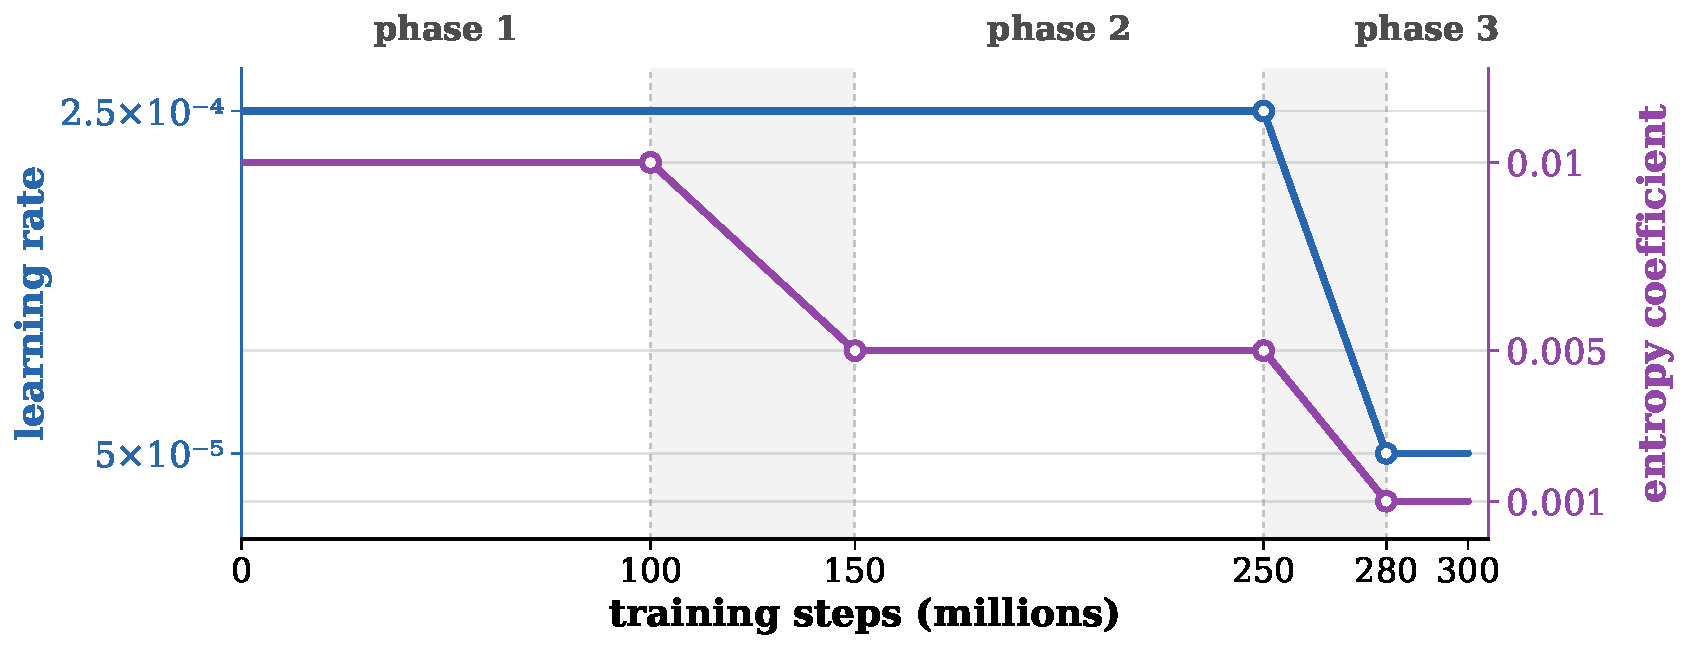
\includegraphics[width=\textwidth]{chapters/10_results/figures/phased_schedule.pdf}
  \caption[Phase schedule for the $300\,\text{M}$-step run]{Phase schedule for the $300\,\text{M}$-step reward-scheduling run: learning rate $\alpha$ and entropy coefficient $\beta$ across the three training phases, linearly interpolated between adjacent phases.}
  \label{fig:phased-config}
\end{figure}

Figure~\ref{fig:rush-collapse} traces evaluation win rate, average episode length, and unweighted per-component returns over $300\,\text{M}$ steps, highlighting the shaped-weight annealing window.

\begin{figure}[!htb]
  \centering
  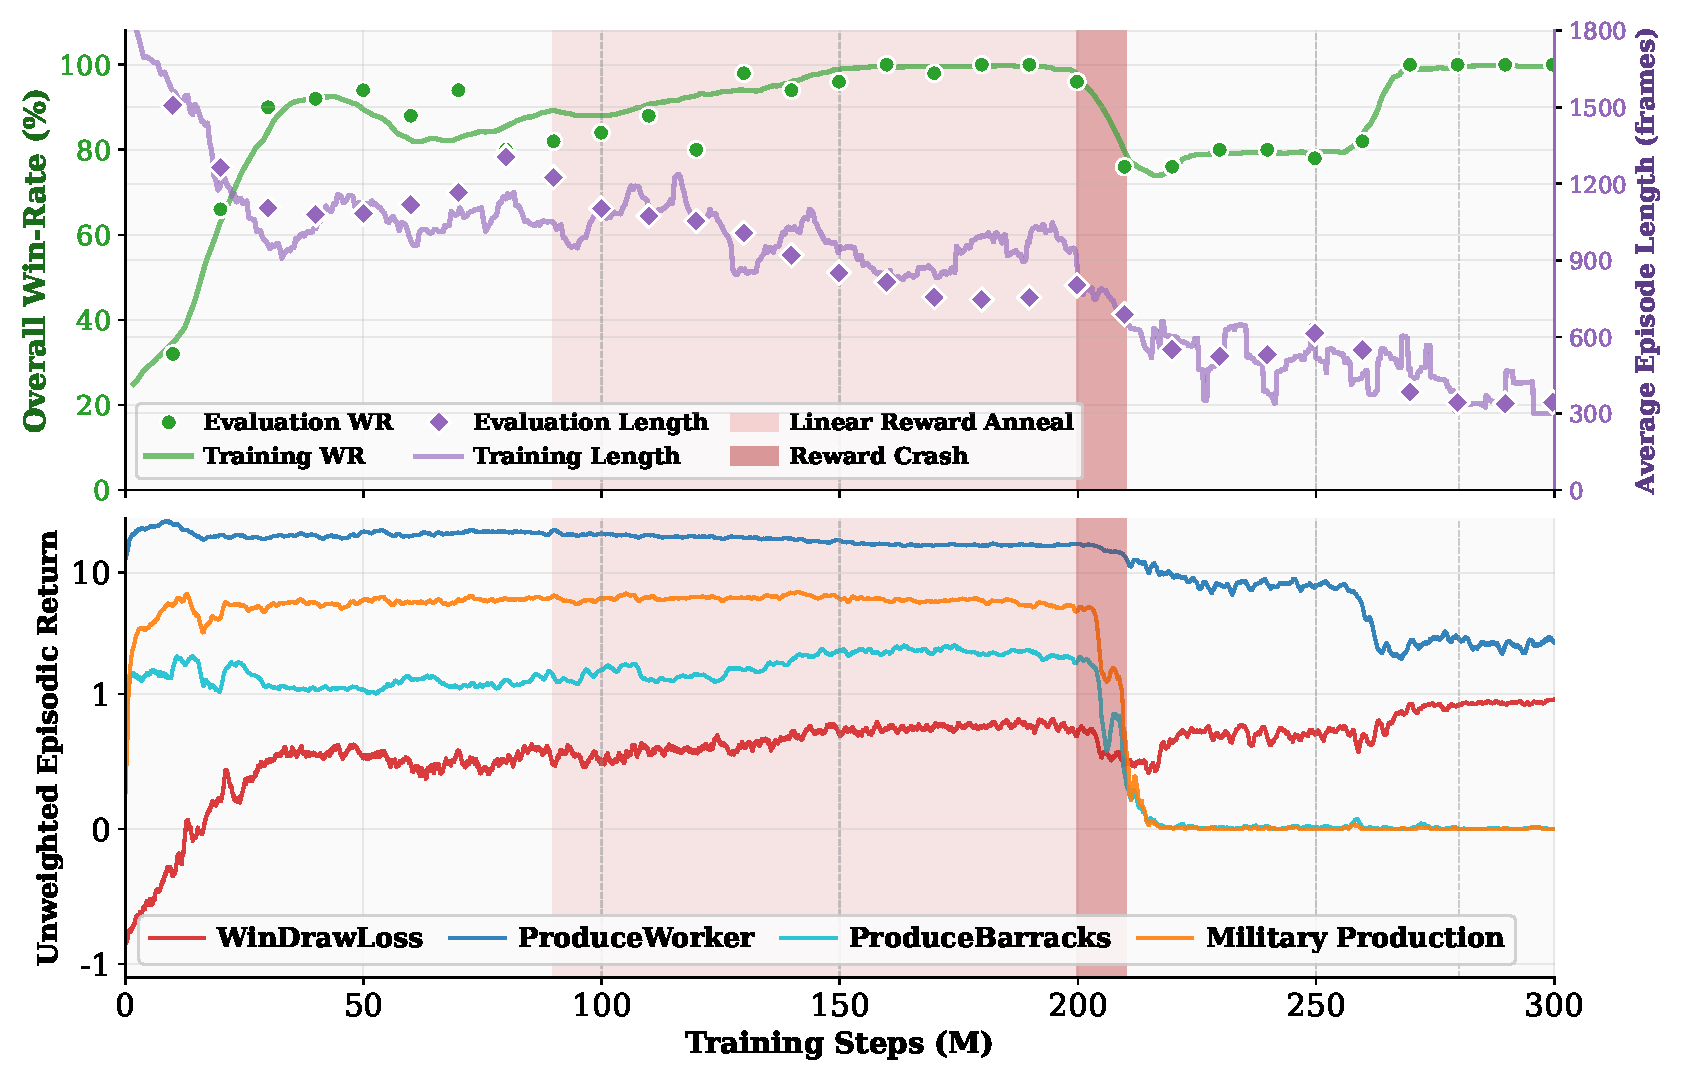
\includegraphics[width=\textwidth]{chapters/10_results/figures/rush_collapse.pdf}
  \caption[Discount-induced rush collapse]{Rush collapse over the $300\,\text{M}$-step reward-scheduling run. \textit{Top:} evaluation win rate (green) and average episode length (purple). \textit{Bottom:} unweighted per-component returns on symlog scale (\textit{WinDrawLoss}, \textit{ProduceWorker}, \textit{ProduceBarracks}, \textit{MilitaryProduction}). Light red marks the shaped-weight annealing window $[90, 210]\,\text{M}$ steps, with a darker inner band at the crash.}
  \label{fig:rush-collapse}
\end{figure}

These training dynamics separate into two regimes. Up to ${\approx}200\,\text{M}$ steps, the agent develops a balanced strategy: evaluation win rate climbs steadily toward $100$\%, episode length stabilizes around $750$ frames, and all reward components rise in concert. After $w_{\text{shape}}$ reaches zero near $210\,\text{M}$, evaluation win rate dips to ${\approx}75$\% before recovering to near-$100$\% by $280\,\text{M}$, while episode length collapses from ${\approx}750$ to ${\approx}300$ frames and the macroeconomic and military components of the return (\textit{ProduceBarracks}, \textit{MilitaryProduction}) fall to zero. The recovery is illusory. The agent has abandoned the strategic components of its policy and is winning by rushing the opponent with its starting workers, a strategy that exploits a short-horizon vulnerability of the training pool. The question is why a policy that had converged to a balanced strategy at $200\,\text{M}$ steps abandons it within the following $90\,\text{M}$ steps, precisely as the shaped reward is removed.

\subsubsection{The Discount-Induced Shortcut}

The collapse is mechanical rather than behavioral: it follows directly from the structure of the discounted-return objective once the shaping signal has been annealed away. Within a trajectory $\tau = (s_0, a_0, r_1, \dots, s_T)$, the episodic return decomposes as
\begin{equation}
G(\tau) \;=\; w_{\text{shape}} \sum_{t=0}^{T-1} \gamma^{t}\, r^{\text{shape}}_{t+1} \;+\; w_{\text{term}}\, \gamma^{T-1}\, r^{\text{term}}_{T},
\label{eq:rush-decomp}
\end{equation}
where $w_{\text{shape}}$ is the shaped-reward weight (annealed linearly), $r^{\text{shape}}_{t}$ are the dense per-step shaping rewards, $w_{\text{term}} = 10$ is the terminal-reward weight, $r^{\text{term}}_{T} \in \{-1, 0, +1\}$ is the terminal win\,/\,draw\,/\,loss signal, $T$ is the policy-dependent episode length, and $\gamma = 0.99$.

\paragraph*{The collapsed objective.}

The agent enters the annealing window already proficient: at $90\,\text{M}$ steps, before $w_{\text{shape}}$ begins to drop, it wins between $80$\% and $90$\% of its games against the training pool, so $r^{\text{term}}_{T}$ is strongly positive in expectation. As $w_{\text{shape}}$ is driven to zero, the shaped sum in Equation~\ref{eq:rush-decomp} vanishes and the PPO objective collapses to
\begin{equation}
J(\pi) \;\xrightarrow{w_{\text{shape}} \to 0}\; w_{\text{term}}\, \mathbb{E}_{\tau \sim \pi}\!\left[\gamma^{T-1}\, r^{\text{term}}_{T}\right] \;\approx\; 10\, \mathbb{E}_{\tau \sim \pi}\!\left[\gamma^{T-1}\right].
\label{eq:collapse-objective}
\end{equation}
Because $\gamma < 1$, the function $T \in \mathbb{N} \mapsto \gamma^{T-1}$ is strictly decreasing, so the optimal policy under Equation~\ref{eq:collapse-objective} is the one that minimizes $\mathbb{E}_{\pi}[T]$, independently of any quality-of-play criterion. Faster wins are not merely preferred; they become the only direction in which the surrogate objective can grow.

\paragraph*{Transfer to PPO-Clip.}

Equation~\ref{eq:collapse-objective} is a statement about the abstract objective $J(\pi)$. The question is how this abstract bias gets transmitted to the actual policy parameters during training. The transmission goes through the empirical advantage. PPO does not optimize $J(\pi)$ directly; it optimizes the clipped surrogate $L^{\text{CLIP}}(\theta)$ introduced in Equation~\ref{eq:ppo-clip}, whose two key quantities for the rush collapse are the empirical advantage $\hat{A}_t$, which carries the bias into the gradient, and the clip operator, which fails to suppress it.

\vspace*{0.1cm}

\textit{\textbf{The advantage carries the bias.}} Once $w_{\text{shape}} = 0$, the only non-zero reward in a trajectory is the terminal one, so the return-to-go from state $s_t$ along a trajectory of length $T$ simplifies to
\begin{equation*}
G_t^{(T)} \;=\; 10\, \gamma^{T-t-1}\, r^{\text{term}}_{T},
\end{equation*}
and the empirical advantage is $\hat{A}_t = G_t - V(s_t)$. The key point is that $V(s_t)$ is a function of state only: it does not depend on the trajectory that follows $s_t$. Comparing two rollouts that share state $s_t$ but end at $T$ and $T - \Delta$, the same $V(s_t)$ is subtracted from both returns, so the difference between their advantages is exactly the difference between their returns:
\begin{equation}
\hat{A}_t^{(T-\Delta)} - \hat{A}_t^{(T)} \;=\; G_t^{(T-\Delta)} - G_t^{(T)} \;=\; \left(\gamma^{-\Delta} - 1\right) G_t^{(T)} \;>\; 0.
\label{eq:advantage-diff}
\end{equation}
Equation~\ref{eq:advantage-diff} is the bridge from the return ratio to the gradient: at every state visited by both trajectories, the action that led to the shorter rollout receives a strictly larger empirical advantage than the action that led to the longer one, irrespective of where $V(s_t)$ sits. The gap grows exponentially with $\Delta$: a one-step shortening multiplies the base return by $\gamma^{-1} \approx 1.01$, and the effect compounds across the remaining horizon.

\vspace*{0.1cm}

\textit{\textbf{The clip does not suppress it.}} Inspecting Equation~\ref{eq:ppo-clip}, the clip operator restricts $\rho_t$ to $[1-\epsilon, 1+\epsilon]$, but $\hat{A}_t$ enters the loss as an unclipped multiplier. PPO's clipping therefore controls only how aggressively the policy is allowed to shift per minibatch in response to a given advantage; it places no bound on how large that advantage can be. As trajectories shorten and $\hat{A}_t$ inflates according to Equation~\ref{eq:advantage-diff}, the gradient $\nabla_\theta L^{\text{CLIP}}$ grows accordingly, and each minibatch update moves the policy toward whatever actions produced the largest empirical advantages, which in the collapsed regime is mechanically the actions that led to the shortest episodes.

\paragraph*{Numerical magnitude.}

Under the run's actual numbers, the amplification is substantial. Shortening the expected episode length from $T_{\text{eq}} \approx 750$ frames (the pre-collapse equilibrium) to $T_{\text{rush}} \approx 300$ frames (the post-collapse rush) amplifies the discounted terminal signal by
\begin{equation}
\frac{\gamma^{T_{\text{rush}} - 1}}{\gamma^{T_{\text{eq}} - 1}} \;=\; \gamma^{T_{\text{rush}} - T_{\text{eq}}} \;=\; \gamma^{-450} \;=\; 0.99^{-450} \;\approx\; 92.
\label{eq:amplification}
\end{equation}
A two-orders-of-magnitude differential between a normal-length win and a fast rush is more than enough to override whatever residual signal the value network had learned during the shaped phase. The per-component returns of Figure~\ref{fig:rush-collapse} make this explicit: \textit{WinDrawLoss} keeps climbing as the agent gets better at the shorter game, while \textit{ProduceBarracks} and \textit{MilitaryProduction} fall to zero and \textit{ProduceWorker} drops from ${\approx}13.0$ to ${\approx}3.0$, because the discounted objective no longer rewards them.

\paragraph*{Conditions and mitigation.}

The pathology arises from three interacting conditions: (i) a discount factor $\gamma < 1$, which makes $\gamma^{T-1}$ sensitive to episode length; (ii) a near-terminal-only reward regime, produced by the shaped weight reaching zero; and (iii) policy control over $T$, which gives the optimizer a route to amplify the terminal signal by choosing shorter trajectories. Mitigation can target any of the three: raising $\gamma$ toward $1$ flattens $\gamma^{T-1}$ across feasible $T$; preserving a non-zero shaping floor maintains a dense per-step gradient that dominates the discounted-terminal one; and an undiscounted average-reward formulation removes the dependence entirely. The remedy adopted in Section~\ref{sec:two-phase-finetuning} follows the second route: the shaped-weight floor is raised from $0$ to $0.1$, restoring a productive-action gradient strong enough to anchor the optimizer to balanced play.

\subsubsection{Out-of-Distribution Cost}

Whether the post-collapse policy is genuinely competent or merely exploits a training-pool weakness can be settled empirically by testing it against opponents the agent never saw. Figure~\ref{fig:rush-fragility} compares the agent at $150\,\text{M}$ steps (the pre-collapse balanced policy) with the agent at $300\,\text{M}$ steps (the post-collapse rush) against the two strongest in-training opponents (CoacAI, Mayari) and two scripted CoG competitors withheld from training (TMA, ObiBotKenobi). If the rush were a transferable strategy, it would hold against both; if it were a shortcut tied to the training distribution, it would hold on the first pair and collapse on the second.

\begin{figure}[!htbp]
  \centering
  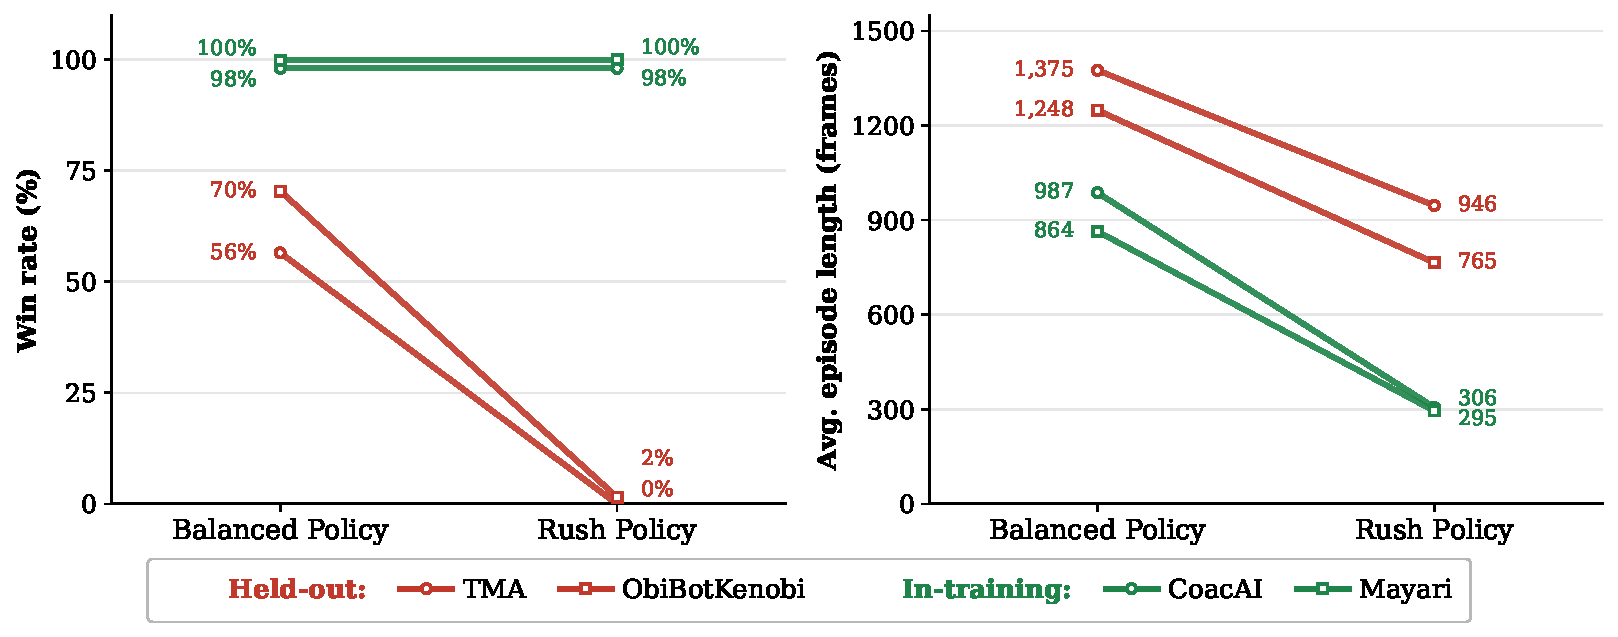
\includegraphics[width=\textwidth]{chapters/10_results/figures/rush_fragility.pdf}
  \caption[Rush fragility on held-out opponents]{Win rate and average episode length (frames) for the $150\,\text{M}$ (balanced policy) and $300\,\text{M}$ (rush policy) checkpoints. The rush matches the balanced policy on in-training opponents (green) but collapses on held-out ones (red).}
  \label{fig:rush-fragility}
\end{figure}

On in-training opponents, the two checkpoints are indistinguishable on win rate (${\sim}98$--$100$\% for both); the only signature of the strategy change is the drop in average episode length from ${\sim}900$ to ${\sim}300$ frames. On held-out opponents, the picture inverts: $\mathrm{WR}$ collapses from $56$--$70$\% to near zero, while episode lengths fall from ${\sim}1\,300$ to ${\sim}850$ frames, well above the ${\sim}300$ frames of a successful rush. The rush is attempted but fails: early worker aggression that broke CoacAI and Mayari is dismantled by opponents with more robust early-game defenses.

This is the empirical signature of the discount-induced shortcut. Against held-out opponents, neither pillar of the rush incentive holds: the rush does not produce a fast win, and many attempts terminate in losses. The shortcut is selected for by the training distribution and collapses against everything else. All subsequent runs therefore retain a $10$\% shaped-reward floor throughout training; this residual signal keeps the value function calibrated and the policy macro-oriented while the dominant gradient contribution still comes from the win\,/\,loss reward.

\subsection{Two-Phase Opponent-Pool Fine-Tuning}
\label{sec:two-phase-finetuning}

Fine-tuning runs in two phases of $24$ environments from the $150\,\text{M}$ checkpoint, with progressively stronger opponents and annealed learning rate, entropy, and shaped weight (Table~\ref{tab:finetune-config}).

\vspace{-0.2cm}

\begin{table}[!htp]
\centering
\caption[Two-phase fine-tuning schedule]{Two-phase fine-tuning schedule from the $150\,\text{M}$ checkpoint to the final \code{UECD-Best} agent. Values interpolate linearly between phase endpoints.}
\label{tab:finetune-config}
\small
\begin{tabularx}{\textwidth}{@{}l >{\centering\arraybackslash}X c >{\centering\arraybackslash}X c >{\centering\arraybackslash}X@{}}
\toprule
 & \textbf{150\,\text{M}} & \textit{Phase 1} & \textbf{240\,\text{M}} & \textit{Phase 2} & \textbf{350\,\text{M}} \\
\midrule
Learning rate & $5 \times 10^{-5}$ & $\longrightarrow$ & $2 \times 10^{-5}$ & $\longrightarrow$ & $9.5 \times 10^{-6}$ \\
Entropy coef. & $5 \times 10^{-3}$ & $\longrightarrow$ & $2 \times 10^{-3}$ & $\longrightarrow$ & $1.2 \times 10^{-3}$ \\
Shaped weight & $1.0$              & $\longrightarrow$ & $0.25$             & $\longrightarrow$ & $0.10$ \\
\bottomrule
\end{tabularx}
\end{table}

\vspace{-0.2cm}

\paragraph{Phase 1: broaden the opponent pool (150\,\text{M} $\to$ 240\,\text{M}).}

The three weakest scripted bots (RandomBiasedAI, WorkerRush, LightRush) are replaced by two competition-level opponents, TMA and ObiBotKenobi, at $2$ environments each. Self-play expands from $12$ to $16$ environments, evenly split between the latest checkpoint and a PFSP-hard sample from the historical pool. By $240\,\text{M}$, the agent reaches near-perfect win rate against all four scripted opponents in the updated pool while preserving the balanced, macro-oriented strategy that the $10$\% shaped-reward floor maintains.

\paragraph{Phase 2: harden against RAISocketAI (240\,\text{M} $\to$ 350\,\text{M}).}

RAISocketAI joins the bot pool at $4$ environments, with each of the four other opponents reduced to $1$ environment; the self-play allocation is unchanged. This phase tightens the policy against the strongest available opponent and produces the final agent, \code{UECD-Best}.

\paragraph{Compute.}

Total training compute for \code{UECD-Best} amounts to $9.47$ GPU-days of full-run wall-clock on a single RTX 6000 Ada, with a strict marginal cost (on-path segments only) of $7.21$ GPU-days. Table~\ref{tab:uecd-best-compute} decomposes this budget by phase; the progressive slowdown it shows reflects heavier opponent inference as the pool broadens (Phase~1) and shifts to RAISocketAI (Phase~2). The gap between full-run and on-path totals captures wall-clock spent past the branch points at $150\,\text{M}$ and $240\,\text{M}$ on segments ultimately discarded from the final agent's training trajectory. RAISocketAI itself used ${\approx}1.5$\,\text{B} steps over $70$ GPU-days across $8$ maps; of this, ${\approx}500\,\text{M}$ steps and $23.6$ GPU-days were spent on the small-map subset ($\le\!16{\times}16$, including \emph{basesWorkers16x16A}). On this subset specifically, \code{UECD-Best} uses less than half the wall-clock budget ($9.47$ vs $23.6$ GPU-days) and trades breadth for depth: ${\approx}350\,\text{M}$ steps on a single layout against ${\approx}500\,\text{M}$ split across the subset. This compute frugality is also an environmental consideration, keeping the energy footprint modest relative to large-scale RL efforts.

\begin{table}[H]
\centering
\caption[Per-phase training budget for \code{UECD-Best}]{Per-phase training budget for \code{UECD-Best} on
\emph{basesWorkers16x16A} (RTX 6000 Ada).}
\label{tab:uecd-best-compute}
\small
\begin{tabular*}{\textwidth}{@{\extracolsep{\fill}}l c r r r@{}}
\toprule
\textbf{Phase} & \textbf{Steps (M)} & \textbf{Eff.\ SPS}$^{\dagger}$
& \textbf{On-path (hours)}$^{\ddagger}$ & \textbf{Full run (hours)}$^{\S}$ \\
\midrule
From scratch               & $0$--$150$    & $1\,226$ & $34.0$  & $68.5$  \\
Phase 1 (broaden pool)     & $150$--$240$  & $825$    & $30.3$  & $50.0$  \\
Phase 2 (vs RAISocketAI) & $240$--$350$  & $281$    & $108.7$ & $108.7$ \\
\midrule
\multirow{2}{*}{$\sum$} & \textbf{350\,\text{M} steps} &
& \textbf{173.0\,hours} & \textbf{227.2\,hours} \\
                        &                    &
& \textbf{7.21\,days}  & \textbf{9.47\,days}  \\
\bottomrule
\end{tabular*}
\par\vspace{2pt}
\begin{minipage}{\textwidth}
\footnotesize\raggedright
\setlength{\parskip}{1pt}\setlength{\parindent}{0pt}
$^{\dagger}$\,Effective step rate over each segment (segment steps divided by on-path wall-clock).\par
$^{\ddagger}$\,Charges only the steps retained in the final agent.\par
$^{\S}$\,Actual wall-clock of each training run; the from-scratch and Phase~1 runs continue past their branch points ($150\,\text{M}$ and $240\,\text{M}$).\par
\end{minipage}
\end{table}

\paragraph{Why a 10\% floor and not pure sparse.}

A small but persistent shaped signal pins the value function to the same scale throughout training, bypassing the discount-shortcut described in Section~\ref{sec:rush-collapse}. The $10$\% floor is a pragmatic stand-in rather than the principled solution. Two alternatives exist. PopArt~\cite{vanhasseltLearningValuesMany2016} could in principle absorb the magnitude shift, but the shaped$\to$sparse transition is not merely a scale change: it removes entire reward components, fundamentally altering what the value function must predict. PopArt handles non-stationarity in magnitude, not in structure. The cleaner remedy is a multi-head value architecture, with separate heads for the shaped, win\,/\,loss, and cost components (as in RAISocketAI), which absorbs the structural shift by design rather than by floor. Triple value heads were in fact the intended solution here. They appear in the feature ablation under that name (Table~\ref{tab:feat-ablation-summary}), but the result understates their potential: the implementation in use at that time contained bugs that were only resolved after \code{UECD-Best} had been trained. The final configuration therefore falls back on the $10$\% floor: less elegant, but functional and stable.

\subsection{The Emergent Ranged-Only Strategy}
\label{sec:emergent-strategy}

After $350\,\text{M}$ cumulative steps, \code{UECD-Best} converges to a consistent \textit{Ranged-only} composition. The agent assigns three workers to early-game resource gathering (RAISocketAI and most other strong bots use two), funding a faster Barracks followed by continuous Ranged-unit production, then exploits the unit's superior range to kite approaching attackers. Replays show this is the dominant tactic against every opponent in the pool, including those that deploy mixed compositions: Light or Heavy rush patterns get decimated before reaching the Ranged line. A \emph{companion website} hosts $36$ recorded \code{UECD-Best} matchups, the source code, the extended tournament metrics, and the CoG bots archive at \url{https://mathisdelsart.github.io/microrts-drl-uecd-website}.

This behavior is \emph{emergent}. It is not encoded in the reward weights, the architecture, or any explicit shaping term. It is the agent's own answer to the joint optimization problem of (i)~maximizing the win\,/\,loss signal, (ii)~tolerating the $10$\% shaped floor that rewards macro activity, and (iii)~staying robust against the diverse opponent pool seen during fine-tuning.

\paragraph{The single residual weakness.}

The \emph{Ranged-only} build holds against RAISocketAI in the majority of games, but its fast Light rush occasionally pierces it before the Ranged line forms (Light $>$ Ranged in close combat, Figure~\ref{fig:unit-counters}). Two interventions targeted a hybrid Light/Ranged composition, both applied over a transition window and annealed back to baseline: \textbf{\emph{(i)}} reward weights re-shaped to elevate \emph{ProduceLight} and penalize \emph{ProduceRanged}, and \textbf{\emph{(ii)}} the entropy coefficient held at an elevated constant ($\beta = 5 \times 10^{-3}$) to slow re-convergence on a single unit type. Neither shifted the policy meaningfully: the agent returned to its \emph{Ranged-only} build once the modifications annealed away, suggesting that the \emph{Ranged-only} optimum is a strong attractor under the current optimization landscape. A more thorough investigation of reward shaping, opponent curricula, or architectural changes promoting compositional flexibility is left for future work.

\section{Evaluating the Single-Map Agent}
\label{sec:single-map-tournament}

A $19$-agent round-robin tournament on \emph{basesWorkers16x16A} (Chapter~\ref{chap:evaluation-framework}) compares the four RL agents developed in this chapter (\code{UECD-AllFeats} and \code{UECD-TopFeats} from Section~\ref{sec:feat-validation}, \code{UECD-Rushed} from Section~\ref{sec:rush-collapse}, and \code{UECD-Best} from Section~\ref{sec:two-phase-finetuning}) against $15$ competition bots. The $1\,710$ pairwise games ($10$ per matchup, $5$ as P0, $5$ as P1) follow the CoG deterministic-action protocol and completed without crash or timeout across all matchups.

\subsection{Win Rate as the Primary Performance Signal}

Figure~\ref{fig:final-standings} reports the overall ranking. \code{UECD-Best} achieves the top score with $174$ points, $10$ ahead of RAISocketAI ($164$). The lead is not an artifact of including multiple \code{UECD} variants: restricted to external (non-\code{UECD}) agents alone, \code{UECD-Best} still ranks first. The intermediate \code{UECD} checkpoints map directly onto each section's contribution. \code{UECD-TopFeats} ($131$ points), from the feature ablation of Section~\ref{sec:feat-validation}, already places fifth overall. \code{UECD-Best} adds $43$ more points, the measurable gain from the two-phase fine-tuning of Section~\ref{sec:two-phase-finetuning}. \code{UECD-AllFeats} ($110$ points) ranks below \code{UECD-TopFeats}, confirming Section~\ref{sec:feat-validation}'s finding: adding the conditional features on top of the top-$5$ does not improve performance and may slow convergence at this budget. \code{UECD-Rushed} ($98$ points) ranks last among the \code{UECD} variants but still ahead of GridNet ($60.5$ points), the published DRL baseline for MicroRTS~\cite{huangGym$m$RTSAffordableFull2021}. This gap is partly inflated by an asymmetry in how GridNet was trained: it only learned to play as P0 and loses every game when forced into the P1 role, which roughly halves its effective tournament total. Even after doubling GridNet's score to compensate (an upper bound, since P0 skill need not transfer to P1), both \code{UECD-TopFeats} ($131$) and \code{UECD-Best} ($174$) still exceed it, confirming that the architectural and feature contributions of this chapter compound positively over the published baseline. Expressed as tournament win rates, this corresponds to a $+63.06$\,pp improvement, from $33.61$\% for \code{GridNet} to $96.67$\% for \code{UECD-Best}\footnote{Tournament-point totals divided by the maximum ($180$): $60.5/180 = 33.61$\% for \emph{GridNet} and $174/180 = 96.67$\% for \emph{UECD-Best}. After symmetry correction for \emph{GridNet}'s P0-only training (doubled score, ${\sim}67.2$\%), the gap narrows to ${\sim}29$\,pp but remains decisive.}.

\begin{figure}[!htp]
\centering

\includegraphics[width=0.9\textwidth]{chapters/10_results/figures/final_standings.pdf}
\caption[Final tournament standings (single-map, $19$ agents)]{Final tournament standings on \textit{basesWorkers16x16A} across $19$ agents under the CoG deterministic-action protocol ($1\,710$ pairwise games, $10$ per matchup split as $5$ P0 and $5$ P1). Ranking is by total points (win~$=$~$1$, draw~$=$~$0.5$, loss~$=$~$0$); the dashed line marks the $50$\% win-rate threshold.}
\label{fig:final-standings}
\end{figure}

\begin{figure}[!htp]
\centering

\includegraphics[width=0.9\textwidth]{chapters/10_results/figures/h2h_matrix.pdf}
\caption[Head-to-head win-rate matrix (single-map, $19$-agent)]{Head-to-head win-rate matrix, agents ordered by total points (matching Figure~\ref{fig:final-standings}). Each cell shows the row agent's win rate (\%) against the column agent over $10$ games; the color scale runs from red ($0$\%) to blue ($100$\%). Diagonal cells are empty (no self-play).}
\label{fig:h2h-matrix}  
\end{figure}

\medskip
The head-to-head matrix (Figure~\ref{fig:h2h-matrix}) refines this ranking. \code{UECD-Best} wins $100$\% of games against every opponent except WorkerRush ($50$\%) and RAISocketAI ($90$\%). The WorkerRush result is an artifact of the deterministic CoG protocol: when both policies are deterministic, the ten games against a single opponent collapse into two identical replays, one per starting position, so a single positional asymmetry produces the $5$--$5$ split. Under the stochastic protocol used elsewhere in this chapter ($1\,000$ games per matchup), \code{UECD-Best} wins $99.3$\% ($\pm0.5$ pp) against WorkerRush, ruling out a structural blind spot. The RAISocketAI head-to-head, re-evaluated under the stochastic protocol, settles at $65.7$\% ($\pm2.9$ pp): still a clear lead, but tighter than the $9$--$1$ deterministic split suggests\footnote{Confidence intervals are $95$\% Wald intervals on a binomial proportion, $\pm1.96\sqrt{p(1-p)/n}$ with $n=1\,000$ games: $\pm0.5$ pp at $p=0.993$ and $\pm2.9$ pp at $p=0.657$. These capture sampling noise at a fixed checkpoint, not seed-to-seed variance, since \emph{UECD-Best} is a single training run.}. The intermediate UECD rows of the matrix show a consistent pattern: they win against the weaker scripted bots on the right side of the matrix but collapse against the strongest opponents on the left (TMA, ObiBotKenobi, RAISocketAI). This is the same fragility profile diagnosed in Section~\ref{sec:rush-collapse}, now visible across the full opponent pool: the two-phase fine-tuning is what bridges the gap to fully competitive play, not the architecture or feature set alone.

\subsection{Game-Theoretic Metrics as Robustness Checks}
\label{sec:gt-metrics}

The point totals of Figure~\ref{fig:final-standings} can be sensitive to the composition of the opponent pool: adding clones of a weak agent, for instance, would inflate every other agent's score uniformly. To complement the standings, four game-theoretic metrics are computed on the $19{\times}19$ win-rate matrix of Figure~\ref{fig:h2h-matrix}, each capturing a distinct property of the agent's behavior across the pool.

\vspace*{0.15cm}

\noindent The \hlc{gray!12}{Copeland score}~\cite{saariCopelandMethodRelationships1996} counts the signed pairwise wins minus losses, measuring dominance \emph{breadth} regardless of margin; \hlc{gray!12}{\mbox{$\alpha$-Rank}}~\cite{omidshafieiARankMultiAgentEvaluation2019} reports the long-run stationary mass of each agent under an evolutionary invasion dynamic, identifying the strategies hardest to displace; \hlc{gray!12}{Nash averaging}~\cite{balduzziReevaluatingEvaluation2018} solves the win-rate matrix as a zero-sum meta-game and reports the agent's expected payoff against the equilibrium mix, separating dominated strategies from the equilibrium frontier; \hlc{gray!12}{Regret}~\cite{savageTheoryStatisticalDecision1951, balduzziReevaluatingEvaluation2018} measures the gap between each agent's win rate and that of the pool's best response, reported both averaged across opponents (\textit{average regret}) and on the single hardest matchup (\textit{worst-case regret}).

\vspace*{0.15cm}

The mathematical definitions and a four-agent worked example illustrating how the metrics complement one another on the same matrix are deferred to Appendix~\ref{app:game-theory}. Table~\ref{tab:gt-metrics} reports the top-$3$ agents per metric, excluding Nash because its top-$3$ is a perfect tie at score $0$ (discussed below).

\vspace*{-0.15cm}

\begin{table}[H]
\centering
\caption[Top-$3$ agents per game-theoretic metric]{Top-$3$ agents per game-theoretic metric, computed on the $19{\times}19$
win-rate matrix. \emph{$\uparrow \; \equiv$ ``higher is better''} and \emph{$\downarrow \; \equiv$ ``lower is better''}.}
\label{tab:gt-metrics}
\small
\setlength{\tabcolsep}{5pt}
% \renewcommand{\arraystretch}{0.8}
\begin{tabularx}{\textwidth}{@{}l | >{\raggedright\arraybackslash}X r | >{\raggedright\arraybackslash}X r | >{\raggedright\arraybackslash}X r@{}}
\toprule
\textbf{Metric} & \multicolumn{2}{c|}{\textbf{Top \#1}} & \multicolumn{2}{c|}{\textbf{Top \#2}} & \multicolumn{2}{c}{\textbf{Top \#3}} \\
\midrule
Copeland ($\uparrow$)                  & \code{UECD-Best} & $+17$   & RAISocketAI      & $+16$   & TMA        & $+11$   \\
$\alpha$-Rank$^{\dagger}$ ($\uparrow$) & \code{UECD-Best} & $0.339$ & RAISocketAI      & $0.182$ & TMA        & $0.079$ \\
Avg.\ regret ($\downarrow$)            & \code{UECD-Best} & $0.03$  & RAISocketAI      & $0.06$  & UtsImass   & $0.19$  \\
Worst-case regret ($\downarrow$)       & RAISocketAI      & $0.40$  & \code{UECD-Best} & $0.50$  & \emph{Tie} & N/A     \\
\bottomrule
\multicolumn{7}{@{}l@{}}{\footnotesize $^{\dagger}$\,Selection intensity $\alpha = 0.1$, Moran population $m = 50$.}
\end{tabularx}
\end{table}

\vspace*{-0.4cm}
\subsubsection{Dominance Breadth: Copeland Score}

Figure~\ref{fig:copeland-scores} reports the Copeland score of every agent in the tournament. \code{UECD-Best} leads with $+17$, RAISocketAI follows at $+16$, and TMA is third at $+11$. Because the Copeland score reduces each matchup to a sign ($+1$ for a win, $-1$ for a loss) and discards margin, the metric reports \emph{dominance breadth}: the number of opponents an agent beats more often than not, regardless of margin.

\code{UECD-Best}'s score of $+17$ corresponds to beating $17$ of its $18$ opponents head-to-head; the single missing point comes from the WorkerRush deterministic-protocol tie discussed in the head-to-head analysis above, which lands at exactly $50$\% and yields a Copeland contribution of $0$. RAISocketAI's $+16$ comes from the same $17$-win profile, with its single non-win being a pairwise loss to \code{UECD-Best} rather than a draw. The drop of $5$ points down to TMA at the next position reflects the same discontinuity already visible in the leaderboard: two agents sit at the top of the pool, the rest decline progressively from $+11$ down through $-18$ for RandomBiasedAI.

\begin{figure}[!htp]
  \centering
  
\includegraphics[width=\textwidth]{chapters/10_results/figures/copeland_scores.pdf}
  \caption[Copeland scores across the tournament]{Copeland scores on the tournament's $19{\times}19$ win-rate matrix, agents sorted from highest to lowest score.}
  \label{fig:copeland-scores}
\end{figure}

\vspace*{-0.5cm}

\subsubsection{Evolutionary Stability: $\alpha$-Rank}

Figure~\ref{fig:alpha-rank-sweep} traces the $\alpha$-Rank stationary mass of each agent as the selection intensity $\alpha$ varies from $10^{-3}$ to $10^{3}$. Two curves dominate the picture entirely. \code{UECD-Best}'s mass grows monotonically with $\alpha$ and rises toward $1.0$ at high selection pressure, displacing every other strategy out of the population. RAISocketAI traces a single low bell that peaks just below $0.2$ at moderate $\alpha$, where \code{UECD-Best} already sits around $0.45$ (read at a higher selection intensity than the $\alpha = 0.1$ used in Table~\ref{tab:gt-metrics}), before collapsing back to zero as $\alpha$ grows further. No other agent ever separates from zero on the visible scale.
  
What this asymmetry reveals is precisely what the leaderboard alone cannot show. At low $\alpha$, selection is too weak to distinguish strategies, and every agent receives roughly equal stationary mass ($1/19 \approx 0.053$). As $\alpha$ grows, the dynamic favors strategies that resist invasion. \code{UECD-Best} is the unique agent that resists invasion from \emph{every} other strategy in the pool, so its mass grows monotonically toward the full population. RAISocketAI resists invasion from every agent \emph{except} \code{UECD-Best}; at moderate $\alpha$ it accumulates non-trivial mass by dominating the rest of the pool, but at higher selection pressure \code{UECD-Best} invades it and the bell collapses. The seventeen other agents are invadable by multiple opponents from the start, and never accumulate measurable mass.

\begin{figure}[!htp]
  \centering
  
\includegraphics[width=\textwidth]{chapters/10_results/figures/alpha_rank_sweep.pdf}
  \caption[$\alpha$-Rank stationary mass vs selection intensity across the tournament]{$\alpha$-Rank stationary mass as a function of the selection intensity $\alpha$. Each curve tracks an agent's long-run share of the population under the evolutionary invasion process; only the top-$5$ agents are highlighted, the rest grouped at the bottom.}
  \label{fig:alpha-rank-sweep}
\end{figure}

\vspace*{-0.5cm}

\subsubsection{The Non-Exploitable Frontier: Nash Averaging}

Figure~\ref{fig:nash-scores} shows a sharply bimodal distribution. Eight agents tie at exactly $0$ (\code{UECD-Best}, RAISocketAI, TMA, ObiBotKenobi, WorkerRush, and the three other UECD variants), while the remaining eleven sit strictly below, from $-0.100$ for Mayari down to $-0.500$ for the weakest. No agent occupies the intermediate range: the split at zero is clean and binary.

The ties at $0$ are equal best responses to the equilibrium mix~$\mathbf{p}^*$: against an opponent playing optimally, none of them can be exploited. The negative-score agents are dominated: the equilibrium mixture beats them in expectation, so they are never played at equilibrium. All four UECD variants sit on the non-exploitable side, including \code{UECD-Rushed} despite its mid-tournament ranking.

Nash averaging therefore reads the tournament as a structural partition rather than a continuous ranking: a small frontier of non-exploitable strategies separated by a clean discontinuity from the dominated rest of the pool. The other metrics produce a smooth ordering, whereas this one produces a binary one, and both draw the boundary at the same agents.

\begin{figure}[!htbp]
  \centering
  
\includegraphics[width=\textwidth]{chapters/10_results/figures/nash_scores.pdf}
  \caption[Nash equilibrium scores across the tournament]{Nash equilibrium scores on the tournament's $19{\times}19$ win-rate matrix. Eight agents tie at exactly $0$ (the value of the game), forming the equal-best-response frontier; agents with strictly negative scores are dominated strategies, never selected at equilibrium.}
  \label{fig:nash-scores}
\end{figure}

\begin{figure}[!htbp]
  \centering
  
\includegraphics[width=\textwidth]{chapters/10_results/figures/robustness_score.pdf}
  \caption[Worst-case and mean-case robustness across the tournament]{Robustness scores on the tournament's $19{\times}19$ win-rate matrix. Left: worst-case robustness. Right: mean-case robustness. Both quantities equal $1 - r$ where $r$ is the corresponding regret in Table~\ref{tab:gt-metrics}; higher is better in both panels.}
  \label{fig:robustness-score}
\end{figure}

\subsubsection{Robustness to the Best Response: Average and Worst-Case Regret}

Figure~\ref{fig:robustness-score} shows two complementary views of the regret metric, both flipped to robustness (robustness $= 1 - $ regret) so higher is better in both panels. The worst-case view (left) is striking: only RAISocketAI ($0.60$) and \code{UECD-Best} ($0.50$) reach non-zero scores; every other agent sits at exactly $0$. The labels indicate where each agent loses the most ground to the best response in the pool. \code{UECD-Best}'s worst-case is WorkerRush, the deterministic-protocol tie analyzed earlier; RAISocketAI's worst-case is \code{UECD-Best} itself, the matchup where its win rate falls furthest below the best response. The bottom seventeen all hit the floor against \code{UECD-TopFeats}, TMA, or \code{UECD-Rushed}, the opponents the best response decisively beats. The mean-case view (right) recovers a continuous ranking that closely tracks the headline leaderboard, with \code{UECD-Best} ($0.97$) and RAISocketAI ($0.94$) at the top followed by a monotone decline.

\section{Generalization Probes}
\label{sec:gen-probes}

Single-map dominance does not imply broader competence. \code{UECD-Best}'s single-map specialization isolates architectural and training contributions for a clean per-component signal, but leaves open how the resulting policy behaves once the training distribution shifts. Two probes give a first cut at this: a \emph{layout shift} (same size, different topology: \emph{TwoBasesBarracks16x16}) and a \emph{scale shift} (same layout family, larger size: \emph{basesWorkers32x32A}). Each pairing plays $100$ stochastic-sampling games.

\begin{figure}[!htbp]
  \centering
  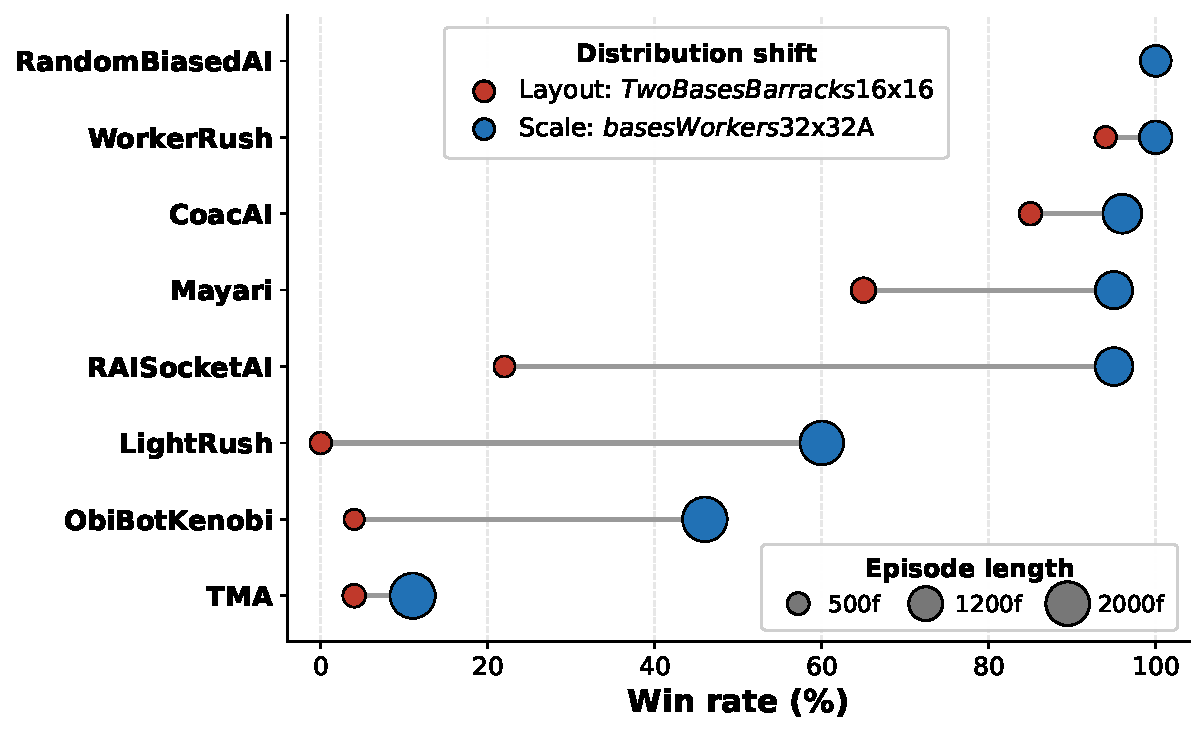
\includegraphics[width=\textwidth]{chapters/10_results/figures/generalization_probes.pdf}
  \caption[Generalization probes: scale and layout shift]{Win rate and mean episode length of \code{UECD-Best} on the two distribution-shift probes against $8$ opponents, over $100$ stochastic-sampling games per matchup.}
  \label{fig:generalization-probes}
\end{figure}

\vspace*{-0.2cm}

Figure~\ref{fig:generalization-probes} reports a striking asymmetry: scale-shift win rate sits well above layout-shift win rate for every opponent, and the gap widens against the strongest agents. The two probes also produce qualitatively different failure modes:

\vspace{0.1cm}

\noindent \hlc{gray!12}{Scale shift is tolerated.} On \emph{basesWorkers32x32A}, the agent retains $\geq 95$\% win rate against $5$ of $8$ opponents (Random, WorkerRush, Mayari, CoacAI, RAISocketAI). The Ranged-only strategy transfers across map size: unit relationships, action semantics, and reward components are unchanged. Where win rate drops (LightRush, ObiBotKenobi, TMA), episode length grows in proportion: the agent loses, but slowly, and still resists instead of collapsing.

\vspace{0.1cm}

\noindent \hlc{gray!12}{Layout shift is brittle.} On \emph{TwoBasesBarracks16x16}, win rate against the strongest opponents collapses (LightRush at $0$\%, ObiBotKenobi at $4$\%, TMA at $4$\%, RAISocketAI at $22$\%). Episode lengths remain short and uniform ($430$ to $650$ frames), with no correlation to win rate: the agent commits early to a strategy that does not match the new topology. Pre-existing Barracks and the second base alter the optimal opening, and \code{UECD-Best} has never seen this configuration.

\vspace{0.1cm}

Taken together, the probes are consistent with a learned representation that encodes map-specific geometric and topological priors rather than transferable strategic invariants: the agent is not perceptually disoriented under either shift, just executing a plan tuned to a different distribution. Several broader conclusions follow plausibly: that single-map training overfits to topology more than to size, that competitive play on a new layout would benefit from per-map fine-tuning or training on diverse layouts, and that scale generalization may emerge more readily from size-aware architectural choices (padded observations, scale-invariant critics). These claims rest on a single test map per shift type and a single trained agent, however, so they remain working hypotheses rather than established results.


\section{Behavior-Cloning Warmstart for PPO}
\label{sec:bc-ppo}

RAISocketAI~\cite{goodfriendCompetitionWinningDeep2024} reported that a single DoubleCone PPO model reached ${\sim}72$\% win rate in the tournament round-robin, while a BC-PPO variant (behavior cloning from bot replays as a warmstart for PPO fine-tuning) reached ${\sim}88$\% on the same benchmark without map-specific fine-tuning. This sizable gap motivates a reproduction of the BC-PPO recipe on the architecture and training pipeline of this thesis to test two hypotheses: \textbf{\emph{(i)}} BC pre-training accelerates convergence during the early steps of PPO, and \textbf{\emph{(ii)}} a BC-initialized PPO reaches a higher final plateau on win rate than from-scratch PPO given equal compute. This section reports a controlled experiment on the single map \emph{basesWorkers16x16A} at $100\,\text{M}$ steps.

\subsection{BC+VF Pre-Training}
\label{subsec:bc-ppo-pretraining}

A script records $\bigl(\mathbf{o}_t, \mathbf{a}_t, r_{t+1}\bigr)$ tuples from \emph{bot-vs-bot} games, observed from one designated bot's perspective. Here, the perspective bot is RAISocketAI and the opponent set is composed of RAISocketAI itself, CoacAI, and Mayari, with $100$ games against each opponent split evenly between positions P0 and P1. This yields $300$ games totaling ${\sim}313\,000$ state-action transitions on \emph{basesWorkers16x16A} (RAISocketAI: ${\sim}161\,000$, CoacAI: ${\sim}86\,000$, Mayari: ${\sim}67\,000$); the imbalance reflects game length, since mirror matches against RAISocketAI last longer.

Following RAISocketAI's formulation, the policy head (cross-entropy on bot actions) and the value head (MSE on discounted reward-to-go) are jointly trained with total loss
\begin{align}
\mathcal{L}_{\text{BC+VF}} = \underbrace{\tfrac{1}{|\mathcal{U}_t|}\sum_{k=1}^{7} \sum_{u \in \mathcal{U}_t} -\log \pi_k\bigl(a_{k,u} \mid \mathbf{o}_t\bigr)}_{\mathcal{L}_{\text{BC}}} \;+\; c_1 \cdot \underbrace{\bigl(V_\theta(\mathbf{o}_t) - G_t\bigr)^2}_{\mathcal{L}_{\text{VF}}},
\label{eq:bc-vf-loss}
\end{align}
where $\mathcal{U}_t$ is the set of active units at step $t$ (the BC loss is per-unit-averaged so that maps with varying army sizes are treated uniformly) and $G_t$ is the reward-to-go of the episode containing $t$. Despite operating on $(\mathbf{o}_t, \mathbf{a}_t, r_{t+1})$ tuples, this stage is not \emph{offline RL}: it involves no Bellman bootstrapping and no policy improvement, and $r_{t+1}$ enters only through the critic's regression target $G_t$. The reward is used as a learning signal only later, by PPO. Pre-training the critic this way, rather than from a random initialization, leaves the value head already informative at the start of fine-tuning and avoids a costly re-bootstrap phase.

\subsection{Comparison Setup}
\label{subsec:bc-ppo-setup}

Both runs use the \code{UECD} architecture and share the same PPO hyperparameters: seed, learning rate, entropy coefficient, parallel environments, total budget ($100\,\text{M}$ steps), and map (\emph{basesWorkers16x16A}). They differ only in initialization: ``BC+VF~$\rightarrow$~PPO'' starts from a BC+VF checkpoint trained for $30$ epochs on the dataset above (with a short $100$-update learning-rate warmup to protect the pre-trained weights), whereas ``From-scratch PPO'' starts from random weights. The from-scratch run is the corresponding architecture-ablation run from Section~\ref{sec:arch-sweep} for this network.

In-training evaluations run every $10\,\text{M}$ steps against five reference opponents (RandomBiasedAI, WorkerRush, LightRush, CoacAI, Mayari), with $10$ games per bot. It is a deliberately light protocol intended to track learning trends, not to support fine pointwise comparisons. The BC+VF checkpoint itself (before any PPO update) is also evaluated against the same five opponents (here with $20$ games per bot) to provide a ``BC-only'' reference.

\subsection{Results and Discussion}
\label{subsec:bc-ppo-results}

Figure~\ref{fig:bc-vs-scratch-overall} summarizes the overall win-rate trajectories.

\begin{figure}[!htb]
\centering
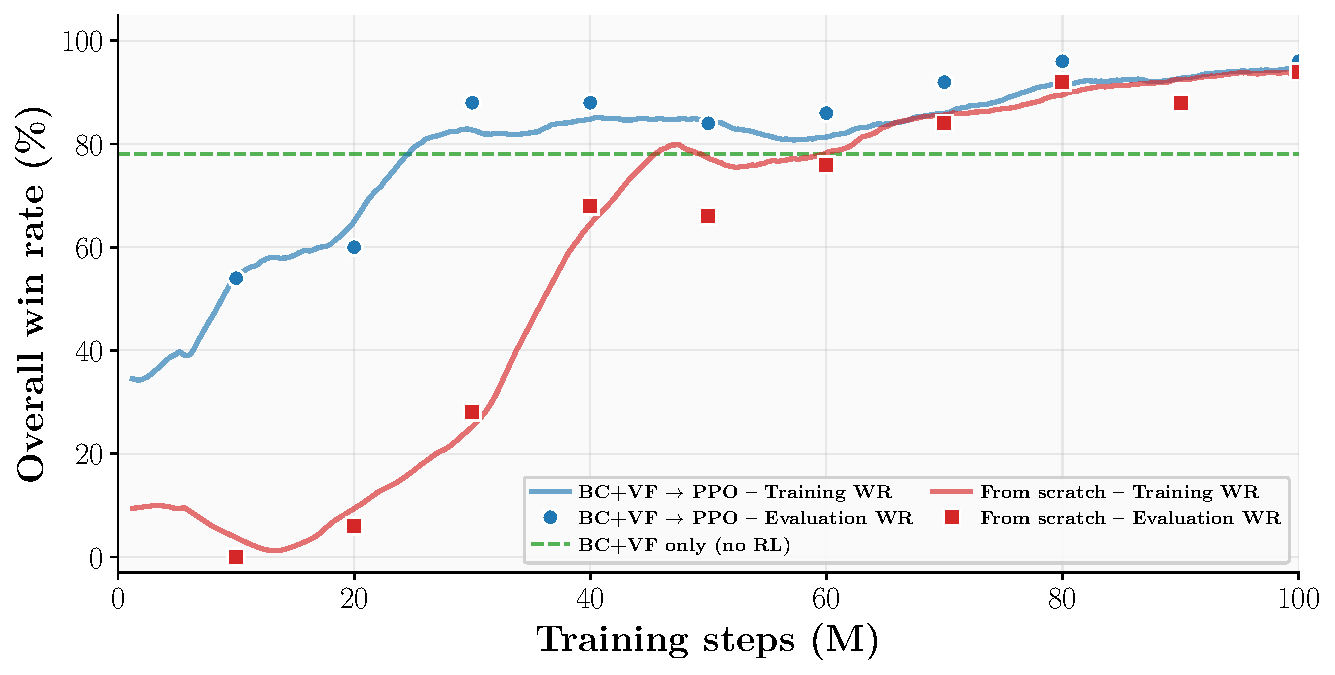
\includegraphics[width=0.9\textwidth]{chapters/10_results/figures/bc_vs_scratch_overall.pdf}
\caption[BC-warmstart vs from-scratch PPO]{Overall in-training win rate against five evaluation bots for BC+VF~$\rightarrow$~PPO (blue) and from-scratch PPO (red) on \emph{basesWorkers16x16A} over $100\,\text{M}$ steps. The dashed green line marks the BC+VF-only reference. Solid lines show the (smoothed) per-episode training $\mathrm{WR}$; markers show evaluation $\mathrm{WR}$ at $10\,\text{M}$-step intervals (points only, not interpolated).}
\label{fig:bc-vs-scratch-overall}
\end{figure}

Three observations stand out. \textbf{\emph{(i)}} ``BC-only'' is already strong: the BC+VF checkpoint alone, trained purely by supervised learning on bot replays, reaches $78$\% overall win rate against the five evaluation bots, confirming that imitating competent bots produces a non-trivial baseline policy. \textbf{\emph{(ii)}} BC strongly accelerates early PPO convergence: at $10\,\text{M}$ steps ``BC+VF~$\rightarrow$~PPO'' has already recovered $54$\% while ``from-scratch PPO'' sits at $0$\% (the from-scratch run has not yet learned basic resource harvesting); the gap is still $+54$ pp at $20\,\text{M}$ and $+60$ pp at $30\,\text{M}$ ($88$\% vs $28$\%), and over the first $50\,\text{M}$ steps the BC run dominates by an average of $41$ pp. \textbf{\emph{(iii)}} No measurable difference at convergence: beyond $70\,\text{M}$ steps both regimes settle in the $84$\% to $96$\% range. The $96$\% vs $94$\% split at $100\,\text{M}$ is well within the binomial noise of a $50$-game evaluation (${\sim}\pm 6$ pp near $95$\% win rate) and should not be read as an asymptotic advantage in either direction\footnote{With $n=50$ games per evaluation point, the standard error (SE) of a binomial proportion is $\mathrm{SE}=\sqrt{p(1-p)/n}\approx0.031$ at $p=0.95$, giving a $95$\% CI of $\pm1.96\,\mathrm{SE}\approx\pm6$ pp. This reflects the sampling noise of one estimate, not a seed-to-seed variance: each run uses a single seed.}.

\medskip

The experiment supports hypothesis~\textbf{\emph{(i)}}: BC pre-training drastically accelerates convergence over the first $50\,\text{M}$ steps. Hypothesis~\textbf{\emph{(ii)}} cannot be cleanly evaluated at this protocol's resolution: at convergence the two regimes sit within the noise of the $50$-game in-training evaluation, so the result is consistent with parity, with a small residual BC advantage, or with a small from-scratch advantage, but not with a large asymptotic gap. A definitive answer would require the $1\,000$-game protocol of Section~\ref{sec:single-map-tournament}, which is not run here. The takeaway is therefore that the value of BC-PPO is \emph{compute-efficiency}: under an unconstrained training budget the from-scratch run has time to catch up, while under tight compute (e.g.\ $100\,\text{M}$ steps on a single GPU) BC produces a significantly stronger agent at equal wall-clock. BC-PPO is reported here as a standalone experiment and is not used by the single-map \code{UECD} agent of Section~\ref{sec:single-map-agent}, which is trained from random initialization.


\section{Multi-Map Agent}
\label{sec:multi-map}

The generalization probes of Section~\ref{sec:gen-probes} showed that a single-map specialist overfits to one topology. The obvious remedy is to train across several maps at once, but before treating that as a result it has to be shown to work at all on the environment stack built for this thesis. This section serves that narrower purpose. Its goal is not to produce a robust or competition-strong generalist, which the remaining compute budget did not allow, but to establish three things: that a single network can be trained across maps of different sizes through the padded environment of Section~\ref{subsec:padding}, that PLR supplies a usable map curriculum, and that the resulting policy spreads its skill across the pool instead of collapsing onto one layout.

\vspace{-0.15cm}

\subsection{Setup}
\label{subsec:multimap-setup}

This experiment produces \code{UECD-MultiMap}, trained from scratch for $200\,\text{M}$ steps on a single RTX~6000 Ada (${\approx} 2.3$ GPU-days), reusing the \code{UECD} architecture and the always-on top-$5$ feature set of Section~\ref{sec:feat-final-selection} (extended observations, filtered masks $+$ reserved observations, MCW, opponent modeling, GELU) without change. Five conditional features are added: \emph{SPP critic}, \emph{frame stack~(4)}, \emph{autoregressive} action sampling, \emph{PAE}, and \emph{PopArt}. The map pool is the five open-competition layouts of size at most $16{\times}16$ (\emph{basesWorkers8x8A}, \emph{FourBasesWorkers8x8}, \emph{NoWhereToRun9x8}, \emph{basesWorkers16x16A}, \emph{TwoBasesBarracks16x16}) (Table~\ref{tab:evaluation-maps}, Appendix~\ref{app:maps}). Every $50$ updates, the training map is resampled by PLR~\cite{jiangPrioritizedLevelReplay2021}, which weights each of the five maps by $(1-\mathrm{WR})$ so the agent spends more time on the layouts where it is currently weakest and less on those it already wins (Section~\ref{sec:generalization}). Self-play, PFSP, and the shaped-to-sparse reward annealing of Section~\ref{sec:two-phase-finetuning} are all left off. All remaining configuration and hyperparameters follow the baseline of Table~\ref{tab:baseline-setup}.

\vspace{-0.15cm}

\subsection{Evaluation}
\label{subsec:multimap-eval}

The evaluation is a round-robin over the five-map training pool against the same competition field as Section~\ref{sec:single-map-tournament}, joined by the single-map champion \code{UECD-Best} of Section~\ref{sec:single-map-agent}, relabeled \code{UECD-SingleMap} below for the specialist-vs-generalist contrast. The tournament runs $6\,000$ games across $16$ agents and five layouts: the fifteen benchmark agents of Tables~\ref{tab:baseline-agents-summary} and~\ref{tab:competition-agents-summary} (except \code{GridNet}, whose fixed $16{\times}16$ critic cannot process the pool's smaller and differently shaped layouts) joined by \code{UECD-SingleMap} and \code{UECD-MultiMap}. The analysis goes from the per-map breakdown carrying the main result, to the home-layout reference exposing the trade behind it, and finally to head-to-head behavior aggregated over the pool.

\vspace{-0.2cm}

\subsubsection{Per-Map Coverage}
\label{subsec:multimap-per-map}

The per-map win rates (Figure~\ref{fig:multimap-winrates}) carry the main result. Forced across maps it never trained on, \code{UECD-SingleMap} collapses on the small layouts, $15$\% on \emph{basesWorkers8x8A} and $26$\% on \emph{NoWhereToRun9x8}, yet peaks at $94$\% on its home \emph{basesWorkers16x16A}, a cross-map standard deviation of ${\approx}28$~pp. \code{UECD-MultiMap} stays between $49$\% and $78$\% on every map, a spread of ${\approx}11$~pp, with no per-map collapse, and finishes well ahead on overall win rate ($64$\% vs $47$\%). Training on the pool converts the specialist's single tall peak into an even, moderate plateau, which is exactly the behavior the padded environment and PLR were meant to enable.

The collapse on \emph{basesWorkers8x8A} is the most informative single data point. There \code{UECD-SingleMap} ranks fourteenth of the sixteen agents, with only LightRush and RandomBiasedAI below it. This nuances the earlier reading of the generalization probes (Section~\ref{sec:gen-probes}). There, scale shift looked tolerable because padding preserved the input geometry. What padding cannot supply is strategy: the near-optimal line on $8{\times}8$ is an immediate worker rush, a behavior the single-map agent never developed on $16{\times}16$. The transferred policy is representationally compatible with the smaller map but strategically unsuited to it, exactly the failure mode the multi-map pool is meant to remove.

\begin{figure}[!htbp]
\centering

\includegraphics[width=0.85\textwidth]{chapters/10_results/figures/multi-maps/winrates_per_map.pdf}
\caption[Per-map win rate over the five-map pool]{Per-map win rate (\%) over the five-map pool, agents ordered by overall standing with the \emph{Overall} column set apart on the right.}
\label{fig:multimap-winrates}
\end{figure}

\vspace{-0.5cm}

\subsubsection{Peak vs Coverage}
\label{subsec:multimap-peak}

The trade behind that plateau is visible on the home map alone (Figure~\ref{fig:multimap-standings-home}). Restricted to \emph{basesWorkers16x16A}, \code{UECD-SingleMap} tops the entire $16$-agent field with $141$ points, ahead of RAISocketAI ($137$), confirming that its specialization is genuine peak strength rather than an artifact of the pooled scoring. \code{UECD-MultiMap} gives up that peak, reaching $82$ points for seventh place on the same map, in exchange for the uniform competence it shows everywhere else. The sixth-place finish is itself a reasonable outcome given that the multi-map run was capped at $200\,\text{M}$ steps split across five layouts, against $350\,\text{M}$ steps spent by \code{UECD-SingleMap} on this single layout.

\begin{figure}[!htbp]
\centering
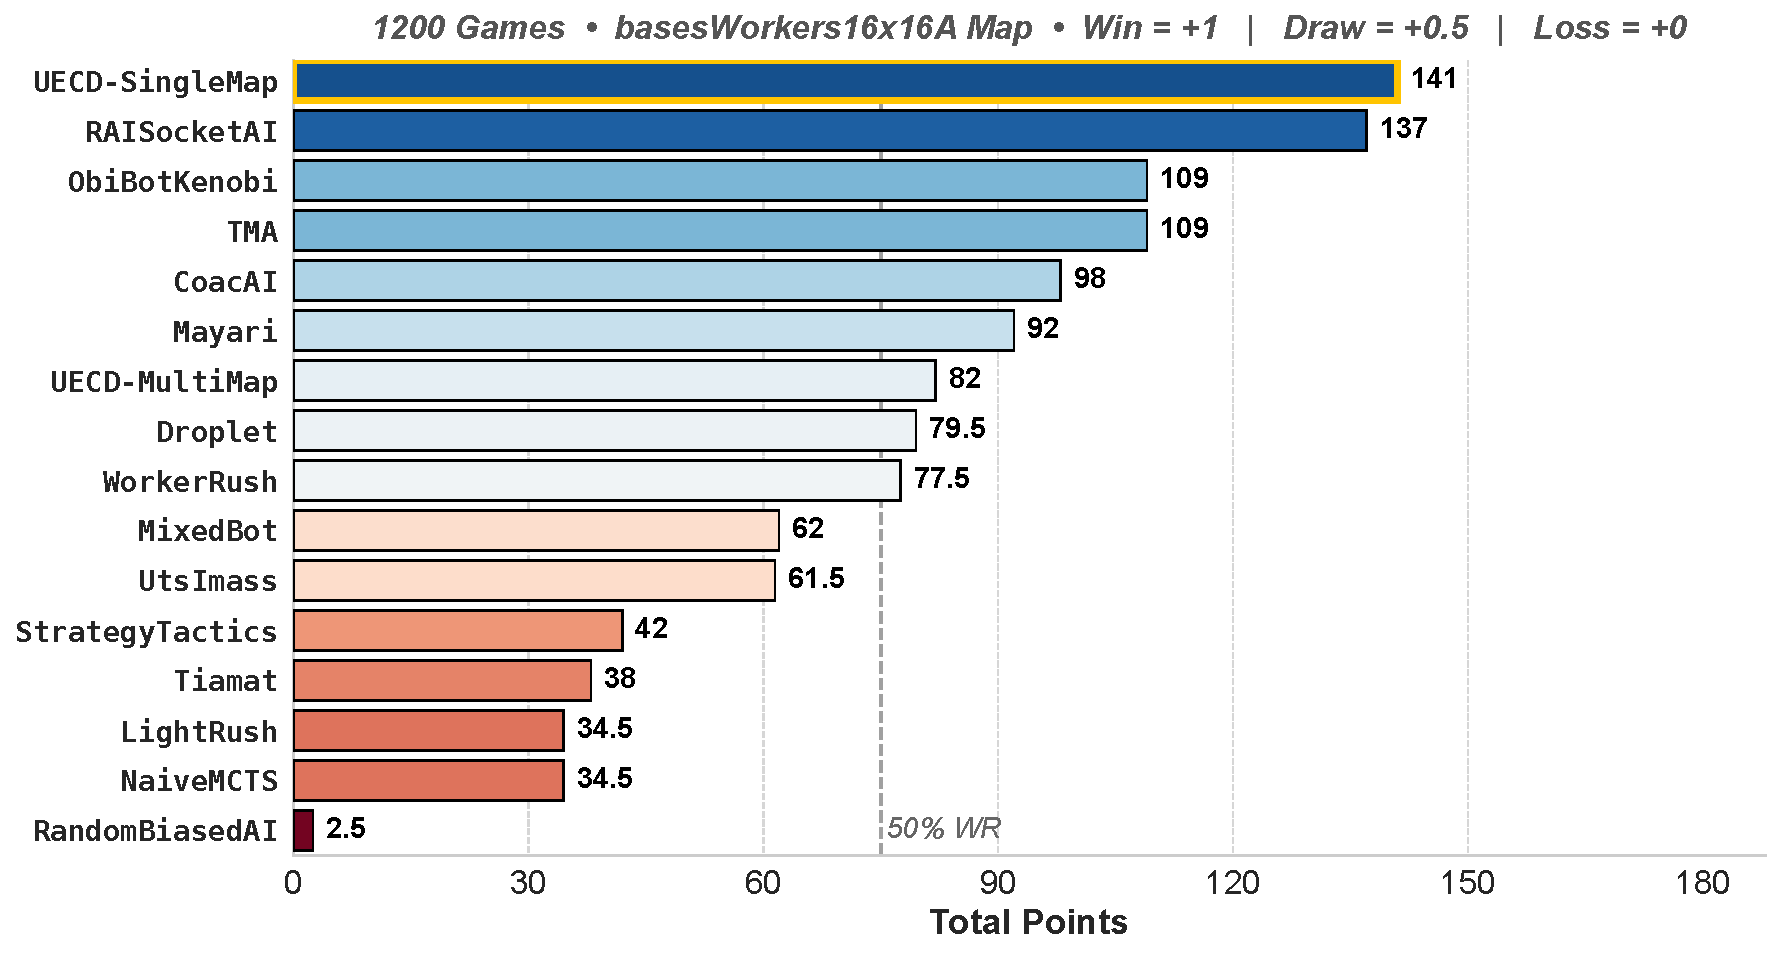
\includegraphics[width=0.9\textwidth]{chapters/10_results/figures/multi-maps/final_standings_baseworker16x16A.pdf}
\caption[Multi-map field: home-map standings]{Final standings on \emph{basesWorkers16x16A} alone ($1\,200$ games), the single layout \code{UECD-SingleMap} (\code{UECD-Best}) was trained on.}
\label{fig:multimap-standings-home}
\end{figure}

\begin{figure}[!htbp]
\centering
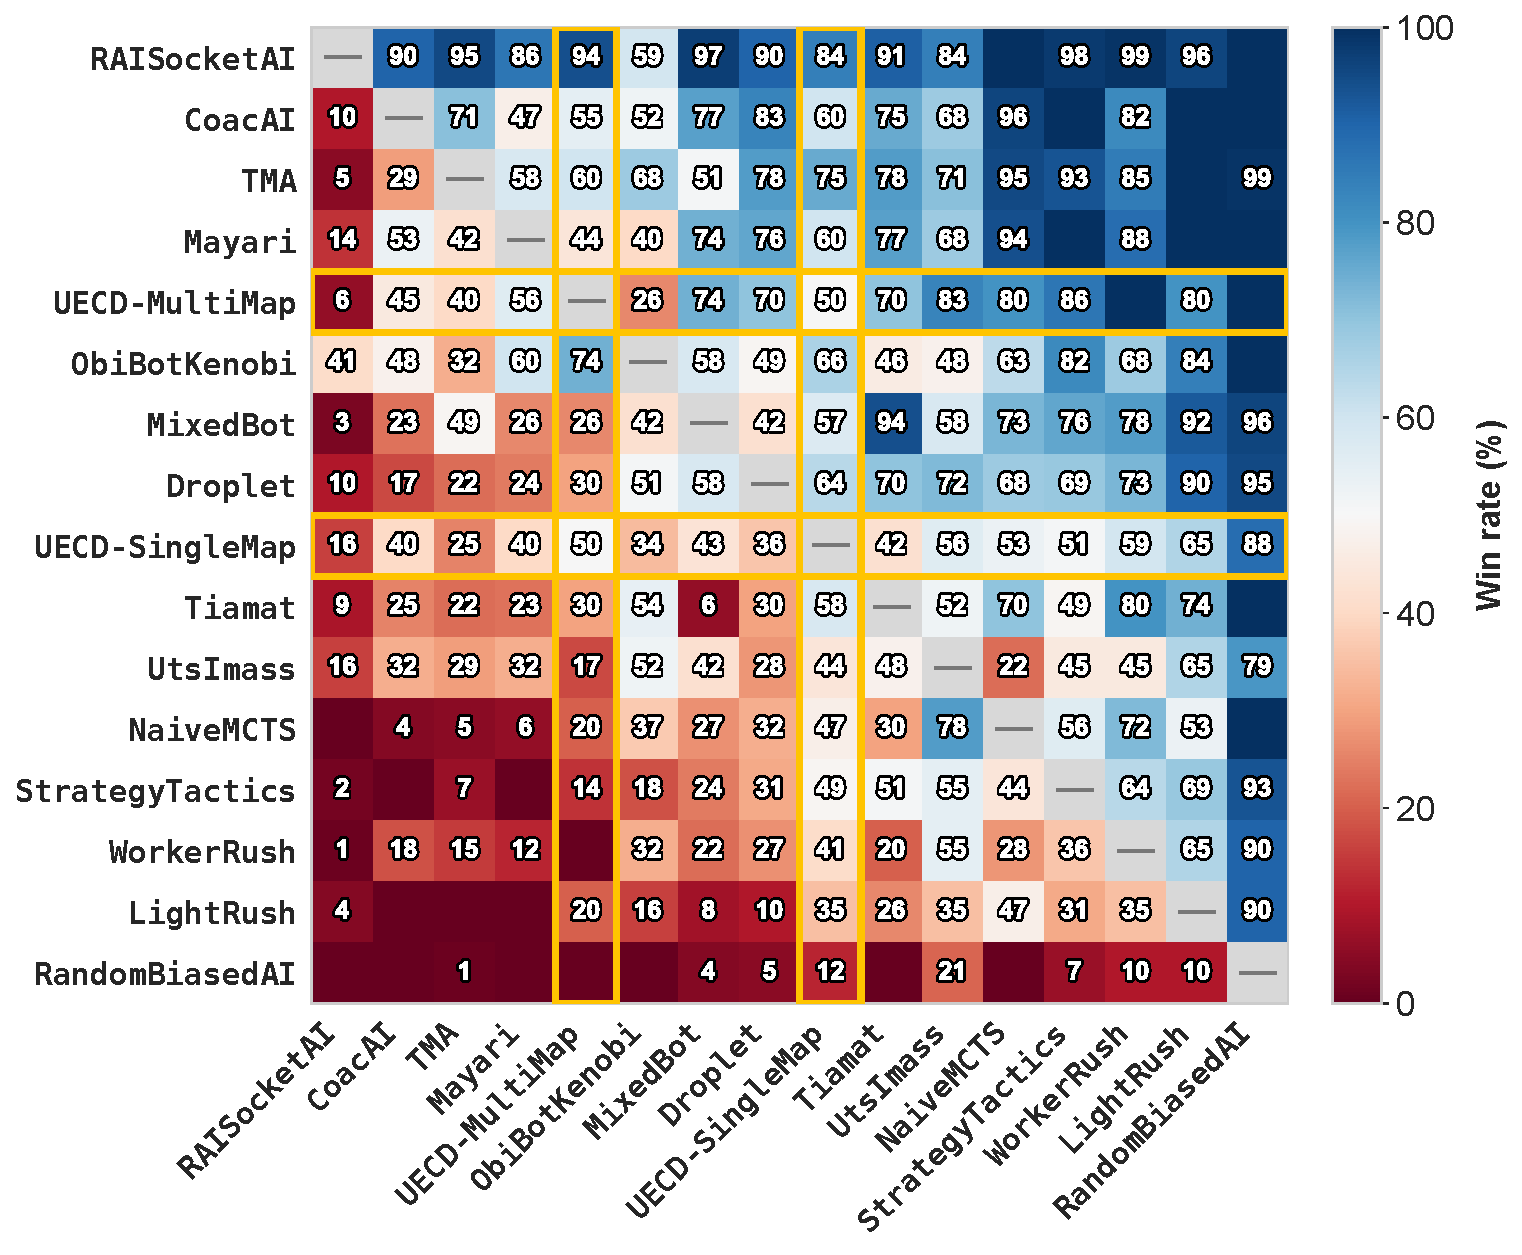
\includegraphics[width=0.9\textwidth]{chapters/10_results/figures/multi-maps/h2h_matrix_global.pdf}
\caption[Global head-to-head win rates (five-map pool)]{Global head-to-head win rates over the five-map pool ($6\,000$ games): cell $(i,j)$ is row~$i$'s win rate against column~$j$, ordered by overall standing, diagonal masked (self-play), \code{UECD} agents bordered in gold.}
\label{fig:multimap-h2h}
\end{figure}

\subsubsection{Head-to-Head over the Pool}
\label{subsec:multimap-h2h}

Aggregated over the pool (Figure~\ref{fig:multimap-h2h}), \code{UECD-MultiMap} wins the majority of its games against every opponent except four: it loses to the three strongest competition bots, RAISocketAI ($2$\%), ObiBotKenobi ($22$\%), and TMA ($40$\%), and splits evenly with CoacAI ($50$\%). It also edges out \code{UECD-SingleMap} head-to-head ($56$\%). \code{UECD-SingleMap}, by contrast, only beats the four weakest agents in the field and trails everyone else. What \code{UECD-MultiMap} gains is robustness of \emph{coverage}: it loses to the same elite bots as the single-map agent, but no longer hands free games to weaker opponents on unfamiliar maps.

\subsection{Hypothesis Assessment}
\label{subsec:multimap-assessment}

The hypothesis was threefold: that a single network can be trained across maps of different sizes through the padded environment of Section~\ref{subsec:padding}, that PLR supplies a usable map curriculum, and that the resulting policy spreads its skill across the pool rather than collapsing onto one layout. The evidence above supports each part. A single unchanged network trained across three map sizes ($8{\times}8$, $9{\times}8$, $16{\times}16$) absorbed the layout diversity without instability; PLR produced a policy with no per-map blind spot; and \code{UECD-MultiMap} spreads competence evenly across the pool, in clear contrast to \code{UECD-SingleMap}. The experiment does not reach competitive peak strength: \code{UECD-MultiMap} still loses to the strongest bots on every map, so this remains a feasibility-and-validation result, not a competition-grade generalist. The price of coverage is a moderate drop on the single-map reference, in line with the reduced budget and the broader objective. The single-map \code{UECD-Best} therefore stands as the stronger headline contribution; the multi-map experiment establishes that broadening the training distribution, not changing the architecture, is the route to generalization, the direction taken up in Chapter~\ref{chap:future-work}.